%%%%%%%%%%%%%%%%%%%%%%%%%%%%%%%%%%%%%%
% yale_thesis.tex
% Elena Gramellini
% Started: 2017/12/05
%
% A bare, sample template for a Yale PhD thesis using yalephd.cls
%%%%%%%%%%%%%%%%%%%%%%%%%%%%%%%%%%%%%%

\documentclass[letterpaper,12pt]{yalephd}
% remove draft option for final printing.
% font size must be between 10pt-12pt.

\usepackage{geometry} % you need this for yalephd.cls to work.
\usepackage{graphicx} % you probably want the rest of these.
\usepackage{dcolumn}
\usepackage{bm}

\usepackage{mathtools}
\DeclarePairedDelimiter\bra{\langle}{\rvert}
\DeclarePairedDelimiter\ket{\lvert}{\rangle}
\DeclarePairedDelimiterX\braket[2]{\langle}{\rangle}{#1 \delimsize\vert #2}

\usepackage{multirow}
\usepackage{amsmath}
\usepackage{amsfonts}
\usepackage{amssymb}
\usepackage{appendix}
\usepackage{comment}
\usepackage{cite}
\usepackage{color}
\bibliographystyle{plain}
\usepackage{slashed}  

\newenvironment{dedication}
  {%\clearpage           % we want a new page          %% I commented this
   \thispagestyle{empty}% no header and footer
   \vspace*{\stretch{1}}% some space at the top
   \itshape             % the text is in italics
   \raggedleft          % flush to the right margin
  }
  {\par % end the paragraph
   \vspace{\stretch{3}} % space at bottom is three times that at the top
   \clearpage           % finish off the page
  }




\begin{document}

% Need to define title before the abstract.
\title{Measurement of the positive kaon-argon total hadronic differential cross section in the LArIAT experiment}
\author{Elena Gramellini}
\advisor{Bonnie T. Fleming}
\date{Date you'll receive your degree} % usually not \today.

% All the stuff at the front of your thesis.
\frontmatter

\begin{abstract}
Abstract goes here. Limit 750 words.
\end{abstract}


\maketitle
\makecopyright{2017}

%  \begin{dedication}
%A mia mamma e mio babbo,\\
%grazie per le radici e grazie per le ali.
%    \par   %% or a blank line
%    \vspace{2\baselineskip}
%To my mom and dad,\\
%thank you for the roots and thank you for the wings.
%    \vspace{\baselineskip}
%  \end{dedication}
\tableofcontents
\listoffigures % remove this if you have no figures.
\listoftables % remove this if you have no tables.

\chapter{Acknowledgements} % this needs to be before \mainmatter.
A lot of people are awesome. But not you, who are reading my thesis before it's done.
%The truth is, younger Elena was a theorists at heart and didn't know. She absolutely loved QFT. But, she hated every single person of her class who self-identified as a theorist. She swore never to become one of them and buried that love deep in her heart, never to be touched by those jerks who traded in Lagrangians and measurements of each other's dicks. Was that love not strong enough to overcome the filth of the everyday shade?  Was she not armored enough to shield from other people?s low self-esteem? Who?s fault was that? Not the theorist?s? she always thought it was hers, but was it?  I don?t know. But sure, younger Elena had to find a way to get by. And she did. Painfully, with a lot of bruises and an ocean across. But she did.

% A big thank you to my academic sisters, a bunch of extraordinary women who have taught me so much on the value
%from the youngest to the oldest (again academically speaking). Supraja, Brooke, the depth of your knowledge, your drive and love for our field is a constant inspiration;  Ariana, thanks for keeping me sane for the last four year, love and hugs to you dudette; and last but not least Xiao, I don't think Fermilab has given me a bigger gift than your friendship. 
% Starts proper arabic numbering of pages and chapters.
\mainmatter

`\chapter{Introduction}\label{ch:-1}

This thesis work concerns the first measurement of the  ($\pi^-$-Ar)  total hadronic cross section  in the 100-1000 MeV  kinetic energy range and the first measurement of the ($K^+$-Ar) total hadronic cross section  in the 100-650 MeV  kinetic energy range. We performed these measurements at the LArIAT experiment,  a small (0.25 ton)  Liquid Argon Time Projection Chamber (LArTPC) on a beam of charged particles at the Fermilab Test Beam Facility.  Albeit particle and nuclear physics have a long history of hadronic cross section measurements, the work outlined in this thesis presents a new methodology -- the ``thin slice method" -- for cross section measurements in argon, possible only thanks to the detection capabilities of the LArTPC technology. The combination of fine-grained tracking and excellent calorimetric information provided by the LArTPC technology  allows to see unprecedented details of particle interactions in argon and, in LArIAT, to measure the kinetic energy of a hadron at each step of the tracking. A renewed interest for precision measurements of hadronic cross sections, particularly in argon, arises from the current  panorama of experimental  particle physics at the intensity frontier.

The discovery of the Higgs boson in 2012 marked the triumph of the Standard Model of Particle Physics; exploring what lays beyond is the real challenge in our field today. 
Since their formulation in 1930, neutrinos have been a source of surprises (and Nobel Prizes) for particle physicists, tiny cracks in our understanding of Nature. In particular, the discovery of neutrino oscillation represents the first evidence of physics Beyond the Standard Model (BSM).  From a theoretical point of view, the field is developing new theories to account for the small but non-zero mass of neutrinos, while trying to remain consistent with the rest of the Standard Model.  From an experimental point of view, we are developing technologies and huge collaborations to probe these theories. As we enter the era of precision measurements of neutrino interaction, neutrinos might hold the key to the next generation of discoveries in particle physics.

Experimentally, precision measurements can be achieved only if the detector technology is able to resolve the fine details of a statistically relevant number of interactions. 
With ``fine details" here we mean the ability to distinguish the many products of the neutrino interaction, such as protons, pions, muons and electrons, and to measure their energy.
Historically,  bubble chamber neutrino detectors were the first revolution in neutrino detection: for example, the spatial resolution of Gargamelle allowed the discovery of neutrino neutral current interaction. Despite the high precision of bubble chambers images, this technology is hard to scale to massive size, making statistical analyses on neutrino interactions almost impossible to perform. To make up for the small neutrino interaction cross section, neutrino experiments moved to very large size, at the expenses of spatial precision. This is the case for the detectors which discovered neutrino oscillation:  both Super-Kamiokande and SNO are massive Cherenkov detectors. With LArTPCs, the field is gaining again bubble-chamber like precision but at massive scales. Following the recommendations of  the latest Particle Physics Project Prioritization Panel  \cite{P5}, the US particle physics panorama is directing a substantial effort towards the exploration of the intensity frontier through the construction of massive LArTPCs. In particular, the near future will see the development of a Short Baseline Neutrino Program (SBN) and long baseline neutrino program  (DUNE), both based on the LArTPC detector technology. The US liquid argon program has the potential to answer many of the fundamental open questions in particle physics today, such as: is there a fourth generation neutrino? is CP violated in the lepton sector? are there any additional symmetries? and, can we find an indication of Grand Unified Theories? 

The SBN program at Fermilab is tasked with conclusively addressing the existence of a fourth neutrino generation in the  $\Delta m^2= \Delta m^2_{14} \sim [0.1 - 10]$ eV$^2$ parameter space. The SBN program entails three surface LArTPCs positioned on the Booster Neutrino Beam at different distances from the neutrino production in oder to fully exploit  the L/E dependence of the oscillation pattern:  SBND (100 m from the decay pipe), MicroBooNE (450 m), and ICARUS (600 m). SBN will also perform an extensive 
program of neutrino cross section measurements, fundamental to abate systematics in the oscillation analyses in both SBN and DUNE.

DUNE has a vast neutrino and non-accelerator physics reach. For what it concerns neutrino physics, oscillation analyses in DUNE have the capability of solving the mass hierarchy and octant problem,  and discovering CP violation in the neutrino sector. Besides its neutrino program, DUNE can open an experimental window on Grand Unified Theories (GUTs). GUTs could potentially answer fundamental questions such as the existence of non-zero neutrino masses and matter-antimatter asymmetry, explaining some ``accidents" in the Standard Models, such as the exact cancellation of the  proton and the electron charge.   Directly probing GUTs at the unification energy scale is impossible by any foreseeable collider experiment. We then need an indirect proof such as baryon number violation, which is predicted by almost every GUT in the form of proton decay, bounded nucleon decay or $n-\bar n$ oscillations on long time-scales. Historically, the main technology used in these searches has been water Cherenkov detectors, with Super-Kamiokande setting all the current experimental limits on the decay lifetimes at the order of $\sim 10 ^{34}$ years. The DUNE far detector and its non-accelerator physics program is a interesting new actor on this stage.  LArTPCs can in fact complement nucleon decay searches in modes where water Cherenkov detectors are less sensitive, especially $p\rightarrow K^+\bar{\nu}$  \cite{Adams:2013qkq}.


Such a diverse physics program speaks to the versatility of the LArTPC technology. LArTPCs provide excellent electron/photon separation \cite{Acciarri:2016sli} lacking in Cherenkov detectors which can be leveraged to abate the photon background from neutral current interactions  in $\nu_e$ searches. LArTPCs also share superb tracking capability with bubble chamber detectors, with several additional benefits. They are electronically read out and self triggered detectors; they provide full 3D-imaging with millimeter resolution, precise calorimetric reconstruction and excellent particle identification. %Plus, female physicists are actually writing code and running experiments, not (only) staring at images \textcolor{red}{-- Too much? --} \cite{2006physics4152G}. 

The amount of information a LArTPC can provide makes these detectors rather complex: a series of dedicated measurements is necessary to obtain meaningful physics results from a LArTPC. The complexity of the LArTPC technology for neutrino detection is due to several reasons. Argon is a fairly heavy element, which means that nuclear effects play an important role in the looks of the interaction topology. For example, pions are one of the main products of neutrino interactions; yet,  since data on charged particle interaction in argon is scarce, neutrino event generators have big uncertainties in the re-scattering simulation of hadrons in argon. %No measurement of hadronic cross sections for pions or kaons is available for argon (yet). 
The amount of details in an LArTPC event is easily  parsed by human eye, but can make automatic event reconstruction rather challenging. Thus, reconstruction algorithms in LArTPC need to be tune to recognize the different topologies of the neutrino interaction products in argon. This is particularly true for pions, since they are an abundant product of the neutrino interactionsl the occurrence of a pion interaction in argon can modify the topology of the neutrino event, causing a misidentification of the neutrino interaction.

The LArIAT \cite{Cavanna:2014iqa} experiment is performing precise cross section measurements of charged particles in argon to bridge this gap of knowledge. 
The LArIAT LArTPC sits on a beam of charged particles at the Fermilab Test Beam Facility; the beam provides charge particles of the type and energy range relevant for neutrino interaction of both SBN and DUNE. The ($\pi^-$-Ar) hadronic cross section is a fundamental input for neutrino detectors in liquid argon, as pion interactions can modify the topology and energy reconstruction of neutrino events in the GeV range, where pion production is abundant. The  ($K^+$-Ar) total hadronic differential cross section in LArIAT is particularly relevant for a high identification efficiency in the context of proton decay searches in DUNE in the  $p\rightarrow K^+\bar{\nu}$  channel. In fact, the kaon-argon cross section affects the kaon topology by modifying the kaon tracking and energy reconstruction, impacting the basis for kaon identification in a LArTPC.  
The cross section analyses exploit the totality of LArIAT's experimental handles; they rely on beam line detector information as well as both calorimetry and tracking in the TPC. These analyses are LArIAT's first physics results. 
In order to measure total hadronic  argon cross sections, several steps are necessary. The analysis starts by identifying a sample of the hadron of interest in the beam line and assessing the beam line contaminations. It proceeds with tracking the hadron candidates in the TPC and measuring their calorimetry at each point in the tracking: the fine sampling of an hadron in the TPC forms the set of ``incident" hadrons.  Then, the hadronic interaction point is identified and the raw cross section is calculated. Two correction\\

This body of work is divided in 8 chapters.
We provide a description of the theoretical framework for the measurements in  Chapter \ref{ch:TheTheory}. Chapter \ref{ch:2} outlines the LArTPC detector technology, while
Chapter \ref{sec:experimentDescription} describes LArIAT experimental setup. We present the event selection for both the pion and kaon analyses, as well as the ``thin-slice method" in Chapter \ref{ch:Interactions}.  Chapter \ref{ch:samples}  describes the work done on the data and Monte Carlo samples in preparation of the cross section analyses.
Chapter \ref{ch:PionXS} shows  the results for the ($\pi^-$-Ar) total hadronic cross section measurement. Chapter \ref{ch:KaonXS} shows  the results for the ($K^+$-Ar) total hadronic cross section measurement. We draw the final remarks on this work in Chapter \ref{ch:Conclusions}

A series of additional studies and calibrations were necessary to perform the cross section analyses. Appendix \ref{ch:AppendixB} shows a measurement of the LArIAT LArTPC electric field using cosmic data. Appendix \ref{ch:AppendixB} shows an optimization of the tracking algorithms geared towards maximizing the efficiency of finding the hadronic interaction point. Appendix \ref{ch:AppendixB} shows the calorimetry calibration of the LArIAT LArTPC, which is a pivotal measurement to enable any physics analysis with TPC data.  



\chapter{Liquid Argon Detectors at the Intensity Frontier}\label{ch:1}


In the next few years, LArTPC experiments -- such as the Short-Baseline Neutrino program (SBN) and DUNE -- will be major players in the intensity frontier field. 

\section{The SBN Program}
\subsection{SBN Goals}
\subsection{Neutrino Interactions and Detection }

\section{DUNE}
\subsection{DUNE Non-Accelerator Physics Program}
\subsection{Rare Decay Searches: Experimental Limit}
\subsection{Nucleon Decay Detection in LAr}

\section{Liquid Argon Time Projection Chambers at the Intensity Frontier}

%Bubble-chamber experiments played a key role in probing the properties of ?-interactions. The Liquid Argon Time Projection Chambers (LArTPC) technology,  first proposed by C.Rubbia in 1977 with ICARUS project [14], is considered the modern evolution of bubble-camber concept, with the additional features of three-dimensional event reconstruction, high-resolution calorimetry, active mass coincident with detector sensitive mass and can intrinsically supply a trigger signal (self-triggering) by means of the scintillation light produced in the liquid noble gas. This technology is ideal to perform $\nu$-studies in a broad energy range, from MeV up to few GeV, with high event reconstruction efficiency, thanks to the capability of particle identifcation and detailed reconstruction of different interaction topologies. In Figure 1.4 is shown a neutrino interaction event, producing a proton, a pion and a muon, as seen in a bubble chamber and in a LArTPC.


\subsection{Time Projection Chamber}
\subsection{Ionization Detectors with Noble Liquids}
\subsection{LArTPC: Principles of Operation}
\subsection{Liquid Argon Ionization Charge Detection}
\subsubsection{Electron Life Time \& purity}
\subsubsection{Space Charge Effect}
\subsubsection{Recombination Effect}
\subsection{Liquid Argon scintillation Light Detection}
\subsubsection{LAr Scintillation Process}
\subsubsection{Wavelength Shifting of LAr Scintillation Light}
\chapter{LArIAT: Liquid Argon In A Testbeam}\label{sec:experimentDescription}
\section{LArIAT \& the Intensity Frontier}
\section{The Particles Path to LArIAT}

LArIAT's home at Fermilab is the Fermilab Test Beam Facility (FTBF), where the experiment 
characterizes a beam of charge particles downstream from the Meson Center beam line. 

LArIAT's particles history begins in the Fermilab accelerator complex with a beam of protons. 
The process of protons acceleration develops in gradual stages, see picture \ref{fig:Accelerator}: gaseous hydrogen is ionized in order to form H$^{-}$ ions; these ions are boosted to 750 keV by a Cockroft-Walton accelerator and injected to the Linac linear accelerator that increases their energy up to 400 MeV; then, H$^{-}$ ions pass through a carbon foil and lose the two electrons; the resulting protons are then injected into a rapid cycling synchrotron, called Booster; at this stage protons reach 8 GeV of energy and are compacted into bunches; the next stage of acceleration is the Main Injector, a synchrotron which accelerates the bunches up to 120 GeV; in the Main Injector, several bunches are merged into one and used for the injection in the last stage.


The Fermilab accelerator complex works in supercycles of roughly 60 seconds in duration. The beam is then split by electrostatic septa and delivered at different experimental halls all over the lab. A 120~GeV$/c$ primary proton beam with variable intensity is extracted in four-second ``spills" and sent to the Meson Center beam line. Here, this primary beam is focused onto a tungsten target to create LArIAT's secondary beam. The composition of the secondary particle beam is mainly positive pions. For the LArIAT data considered in this work the secondary beam peak momentum was fixed at 64~GeV$/c$, although the beam is tunable in momentum between 8-80\,GeV$/c$; this was deemed a secondary beamline configuration which allowed a stable beam operation of the FTBF.
The beam of pions impinges then on a copper target within a steel collimator inside the LArIAT experimental hall (MC7) to create LArIAT tertiary beam, whose geometry in MC7 has been optimized for LArIAT (shown in  Fig.~\ref{fig:tert-layout}).   The steel collimator selects particles produced with a $13^\circ$ production angle at the target down the beamline.  The particles are then bend by  $~10^\circ$  through a pair of dipole magnets.  Tuning the magnets field intensity results in a range of particle momenta from 0.2 to 1.4~GeV/c.
The tertiary beam composition counts mostly pions and protons with a small fraction of electrons, muons, and kaons present as well. It is the job of the LArIAT beamline detectors to select the particles polarity,  to perform particle identification (beamPID) and to measure the momentum of the tertiary beam particles before they get to the LArTPC. The LArIAT detectors are described in the following paragraphs.  

%\begin{comment}     
\begin{figure}
  \centering  	
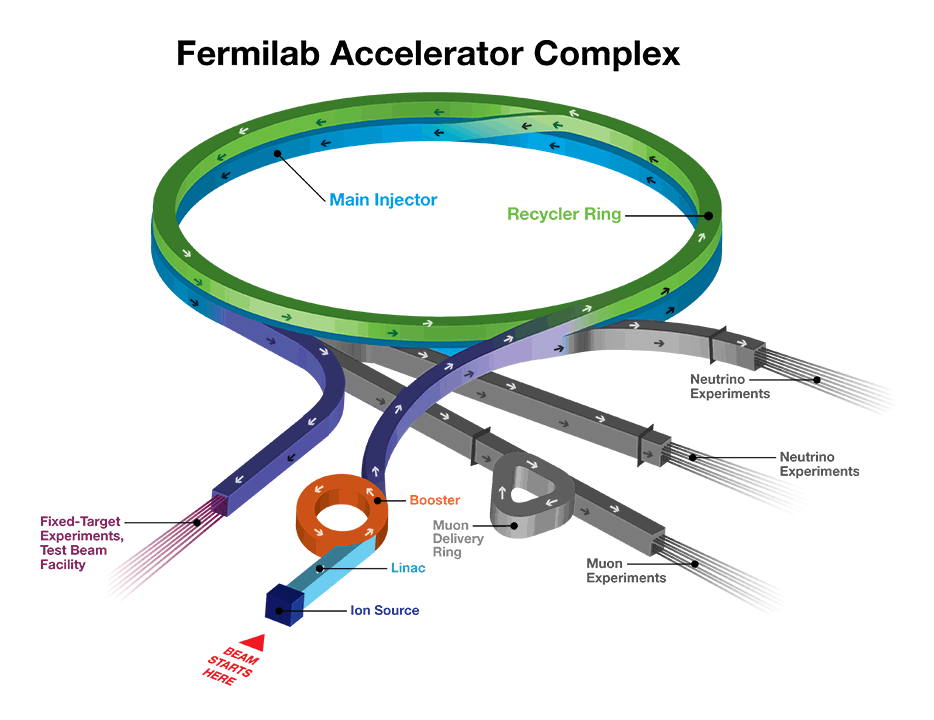
\includegraphics[width=\textwidth,height=\textheight,keepaspectratio]{Chapter-2/Images/AcceleratorFNAL.png}
\label{fig:Accelerator}
\caption{Layout of Fermilab Acellerator complex.}
\end{figure}

%\begin{comment}     
\begin{figure}
  \centering  	
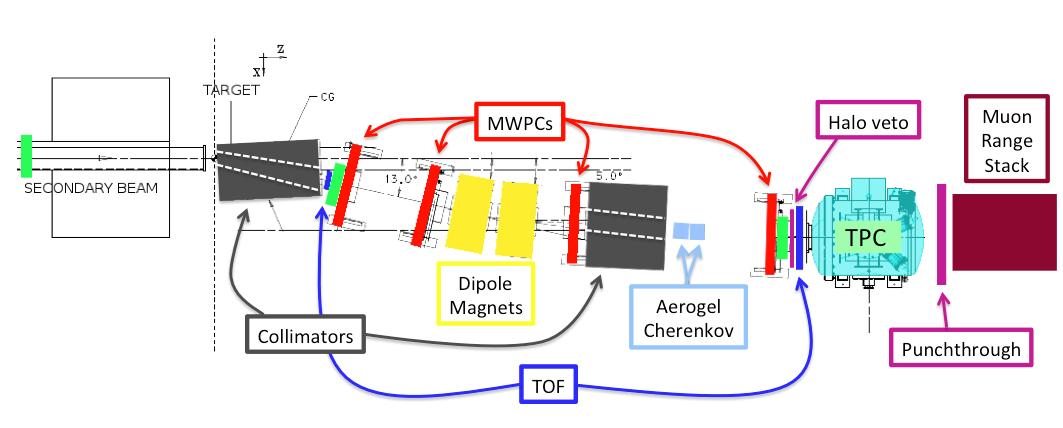
\includegraphics[width=\textwidth,height=\textheight,keepaspectratio]{Chapter-2/Images/Tertiary.png}
\label{fig:tert-layout}
\caption{Birds eye view of the LArIAT tertiary beamline. In grey: upstream and downstream collimators; in yellow: bending magnets in yellow; in red: wire chambers; in blue: time of flight; in green: liquid argon TPC volume; in maroon: muon range statck.}
\end{figure}


%%%%%%%%%%%%%%%%%%%%%%%%%%%%%%%%%%%%%%%%%%%%%%%%%%%%%%%%%%%%
\section{LArIAT Tertiary Beam Instrumentation}\label{sec:Instrumentation}

%%%%%%%%%%%%%%%%%%%%%%%%%%%%%%%%%%%%%%%%%%%%%%%%%%%%%%%%%%%%
The instrumentation of  LArIAT tertiary beam and the TPC components have changed several times during the three years of LArIAT data taking. The following paragraphs describe the components operational during the data taking period relevant to the hadron cross section measurements (a.k.a. Run II).

The components of the tertiary beamline instrumentation key for the hadron cross section analyses are the target and collimators system, the two bending magnets (in a similar configuration used for the  MINERvA T-977 test beam calibration~\cite{MinervaTestbeam}) a set of four wire chambers (WCs) and two time-of-flight scintillating paddles (TOF) and, of course, the LArTPC.  The magnets determine the polarity of the particles in the tertiary beam; the combination of magnets and wire chambers determine the particles momentum, which is used to determine the particle species in conjunction with the TOF.
A muon range stack downstream from the TPC and two sets of cosmic paddles configured as a telescope surrounding the TPC are also used for calibration purposes.


\subsection{Bending Magnets}\label{sec:Magnets}
%%%%%%%%%%%%%%%%%%%%%%%%%%%%%%%%%%%%%%%%%%%%%%%%%%%%%%%%%%%%
LArIAT uses a pair of identical Fermilab type ``NDB" electromagnets, recycled from the Tevatron's anti-proton ring \textcolor{red}{CITE CDF?}. 
The magnets are a fundamental piece of the LArIAT beamline as they are used in all the three tasks of the LArIAT beamline: the sign of the current in the magnet provide the selection of either positively or negatively charged particles, the value of the magnetic field is used in the momentum determination and the subsequent particle identification. 

We describe here the characteristics and response of one magnet. We expect the second one have a similar response, being identical in shape and with a similar history. The magnet aperture measures the gap dimensions to be 14.224~cm of height, 31.75~cm width, and  46.67~cm length.  The wire chambers aperture ($\sim$12.5~cm) is smaller than the magnet aperture, thus, only the central part of the magnet gap is utilized. The field is extremely uniform over this limited aperture and was measured with two Hall probes, both calibrated with nuclear magnetic resonance probes. The probes measured the excitation curve shown in Figure~\ref{fig:magnet_excitation}. 

\begin{figure}[!h]
\begin{centering}
\vspace{-0.3cm}
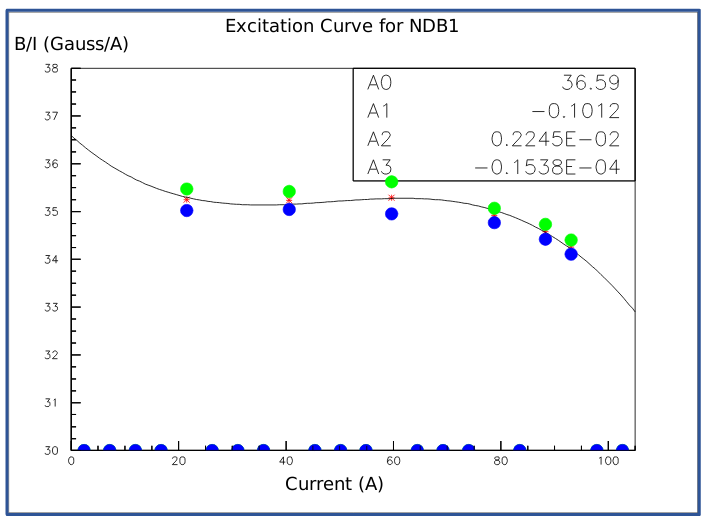
\includegraphics[height=3.0in]{Chapter-2/Images/ExcitationCurves.png}
\caption{
{ Magnetic field over current as a function of the current, for one NDB magnet (excitation curve). The data was collected using two Hall probes (blue and green). We fit the readings with a cubic function (black) to average of measurements (red) given in the legend.}
}
\label{fig:magnet_excitation}
\end{centering}
\end{figure}

The current being passed through the magnets at a given time is identical in both magnets. For Run II period, the current settings explored were 60A (B $\sim$0.21 T) and 100A (B $\sim$0.35 T) in both polarities. 
Albeit advantageous to enrich the tertiary beam composition with high mass particles such as kaons, we never pushed the magnets current over 100 A, not to incur in overheating.  During operation, we operated a air and water cooling system on the magnets and we remotely monitored the magnets temperature.
 
\subsection{Multi-Wire Proportional Chambers}\label{sec:MWPC}
%%%%%%%%%%%%%%%%%%%%%%%%%%%%%%%%%%%%%%%%%%%%%%%%%%%%%%%%%%%%
\begin{figure}[!h]
\begin{centering}
\vspace{-0.3cm}
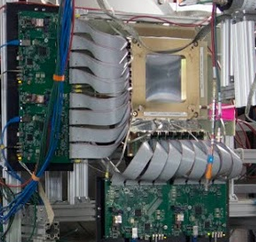
\includegraphics[height=2.3in]{Chapter-2/Images/WireChamber.png}
\caption{
{One of the four Multi Wire Proportional Chambers (WC) used in the LArIAT tertiary beamline.}
}
\label{fig:wirechamber}
\end{centering}
\end{figure}

LArIAT uses four Multi-Wire proportional chambers, or wire chambers (WC) for short, two upstream and two downstream from the bending magnets. The geometry of one chamber is shown in Figure~\ref{fig:wirechamber}: the WC effective aperture is a square of  12.8~cm perpendicular to the beam direction.  Inside the chamber, the 128 horizontal and 128 vertical wires hang at a distance of 1~mm from each other in a mixture of 85\% Argon and 15\% isobutane gas.  The WC operating voltage is between 2400 V and 2500 V. LArIAT wire chambers are an upgraded version of the Fenker Chambers~\cite{Fenker}, where an extra grounding improves the signal to noise ratio of the electronic readout.  

Two ASDQ chips~\cite{ASDQchip} mounted on a mother board plugged into the chamber serve as front end amplifier/discriminator. The chips are connected to a multi-hit TDC~\cite{Sten} which provides a fast OR output used as first level trigger. The TDC time resolution is 1.18~ns/bin and can accept 2 edges per 9~ns.  
The maximum event rate acceptable by the chamber system is of 1 MHz: this rate is not a limiting factor considering that the rate of the tertiary particle beam at the first wire chamber is estimated to be less than 15 kHz. A full spill of data occurring once per supercycle is stored on the TDC board memory at once and read out by a controller specially designed controller.  We use LVDS cables to carry both power and data between the controller and the TDCs and from the controller to the rest of the DAQ.  
%It is possible to program the time window for acceptance for hits, time offsets, front end threshold, and pulse shaping parameters through the controller via a USB from a PC or through an Ethernet connection.

\subsubsection{Multi-Wire Proportional Chambers functionality}\label{sec:MWPCfunc}


\subsection{Time-of-Flight System}\label{sec:TOF}
%%%%%%%%%%%%%%%%%%%%%%%%%%%%%%%%%%%%%%%%%%%%%%%%%%%%%%%%%%%%
Two scintillator paddles, one upstream to the first set of WCs and one downstream to the second set of WCs  form LArIAT  time-of-flight (TOF) detector system. 

 \textcolor{red}{find exact dimentsions}
The upstream paddle is made of a 10 x 6 x \textcolor{red}{?}~cm scintillator piece, read out by two \textcolor{red}{Hamamatsu 2 inch} PMTs mounted on the beam left side which collect the light from light guides mounted on all four edges of the scintillator. The downstream paddle dimensions are  14 x 14 x \textcolor{red}{?}~cm and it is read out by two \textcolor{red}{Hamamatsu 2 inch} PMTs on the opposite ends of the scintillator.
The relatively thin width on the beamline direction minimizes energy loss of the particles coming from the target in the scintillatior material.

\begin{figure}[!h]
\begin{centering}
\vspace{-0.3cm}
%\includegraphics[height=2.3in]{figures/tofdelay.png}
\caption{
{\scriptsize \sf Pictures of the TOF system as was deployed during Run-I and Run-II data taking. The left image is of the upstream TOF paddle and the right image is of the downstream TOF paddle }
}
\label{fig:TOFSystemRunIandII}
\end{centering}
\end{figure}



The CAEN 1751 digitizer is used to digitize the TOF PMTs signals at a sampling rate of 1 GHz. The 12 bit samples are stored in a circular memory buffer. At trigger time, data from the TOF PMTs are recorded to output in a 28.7 $\mu$ second windows starting  approximately 8.4 $\mu$sec before the trigger time. 



\subsubsection{TOF functionality}\label{sec:MWPCfunc}


The TOF signals rise time (10-90\%) is 4 ns and a full width, half-maximum of 9 ns consistent in time. The signal amplitudes from the upstream TOF and  downstream TOF are slightly different:  200 mV for the upstream PMTs but only 50 mV for downstream PMTs. 

The time of the pulses was calculated utilizing an oversampled template derived from the data itself. The pulse pedestal was taken from samples far from the pulse and subtracted to the pulse amplitude. We then stretch vertically a template to match the pedestal-subtracted pulse amplitude and we move it horizontally to find the time. With this technique, we find a pulse time-pickoff resolution better than 100 ps.  The pulse pile up is not a significant problem given the TOF timing resolution and the rate of the particle beam.  Leveraging on the pulses width uniformity of any given PMT (sigma of 400 ps),  we flag events where two pulses overlap as closely in time as 4 ns with an 90\% efficiency according to simulation. 


We combine the pulses from the two PMTs on each paddle to determine the particles' arrival time by averaging the time measured from the single PMT, so to minimize errors due to optical path differences in the scintillator.  However, a time spread of approximately 300~ps is present in both the upstream and downstream detectors, likely due to transit time jitter in the PMTs themselves.  There is no evidence of systematic timing drift over long periods such as 3-4 months of a data-taking: the maximum variation of the average time differences between pairs of PMTs reading out the same scintillator is of the order of 150~ps.



\section{In the Cryostat}

\subsection{TPC: Charge Collection}\label{sec:TPC}
\subsection{TPC: Light Collection System}
\subsection{Cryogenics and Purity Control}
\subsection{TPC: Electric Field Measurement}
\section{Trigger and DAQ}
\section{Control Systems}

\begin{comment}




%%%%%%%%%%%%%%%%%%%%%%%%%%%%%%%%%%%%%%%%%%%%%%%%%%%%%%%%%%%%
\subsubsection{Punch-Through and Muon Range Stack Instruments}\label{sec:MuRS}
%%%%%%%%%%%%%%%%%%%%%%%%%%%%%%%%%%%%%%%%%%%%%%%%%%%%%%%%%%%%


%%%%%%%%%%%%%%%%%%%%%%%%%%%%%%%%%%%%%%%%%%%%%%%%%%%%%%%%%%%%
\subsection{LArIAT Cosmic Ray Paddle Detectors}\label{sec:CosmicRayPaddle}
%%%%%%%%%%%%%%%%%%%%%%%%%%%%%%%%%%%%%%%%%%%%%%%%%%%%%%%%%%%%

LArIAT's system to trigger on cosmic rays is based on two so-called "cosmic towers" which stand  upstream and downstream of the cryostat, one on beam's right and one on beam's left, framing the cryostat.  Each cosmic tower is composed of two paddle assemblies, upper and lower.  The paddle assemblies each consist of four paddles, a matched pair which stand upright and a second matched pair lying across the top  of the assembly, to act as a veto for downward-going cosmic ray air showers.  Unless vetoes by the horizontal paddles, signals from paddle assemblies along the body diagonals of the TPC are combined in a logical ``AND'' to select cosmic muons crossing the TPC along one of its diagonals. A high proportion of events triggered this way contain cosmic ray tracks crossing both anode and cathode.  Such tracks provide a sample of LAr ionization with effectively uniform linear ionization density, but experience the entire range of charge attenuation available in the TPC before they drift to the anode. These tracks are used to calculate and monitor the level of electronegative contaminants in the liquid argon and provide a calibration sample for calorimetry and electric field studies outlined in Section \ref{sec:DetectorPerformance}.

The paddles have trapezoidal shape and are each enclosed in an aluminum case. An example is shown in Fig. \ref{pic:cosmicpaddle}. They come in two different sizes: a smaller version, with bases $32.2~cm$ and $26.7~cm$, $61.0~cm$ height and $3.02~cm$ thickness, and a bigger version, with bases $33.2~cm$ and $27.0~cm$, $70.8~cm$ height and $3.02~cm$ thickness. Each paddle is equipped with wavelength-shifting optical fibers running along one of the long sides and optically coupled to a low voltage, Zener-diode Hamamatsu H5783 PMT.  Signals from the PMT are amplified and discriminated by a custom-made PMT Amplifier and Discrimination (PAD) circuit mounted at one end of the paddle, then sent through a CAT5 cable to a Control and Concentrator Unit (CCU) which both power the PMT, controlling voltage and threshold, and output the PMT signal as logic ECL pulse.

\begin{figure}[h!]
 \centering
% 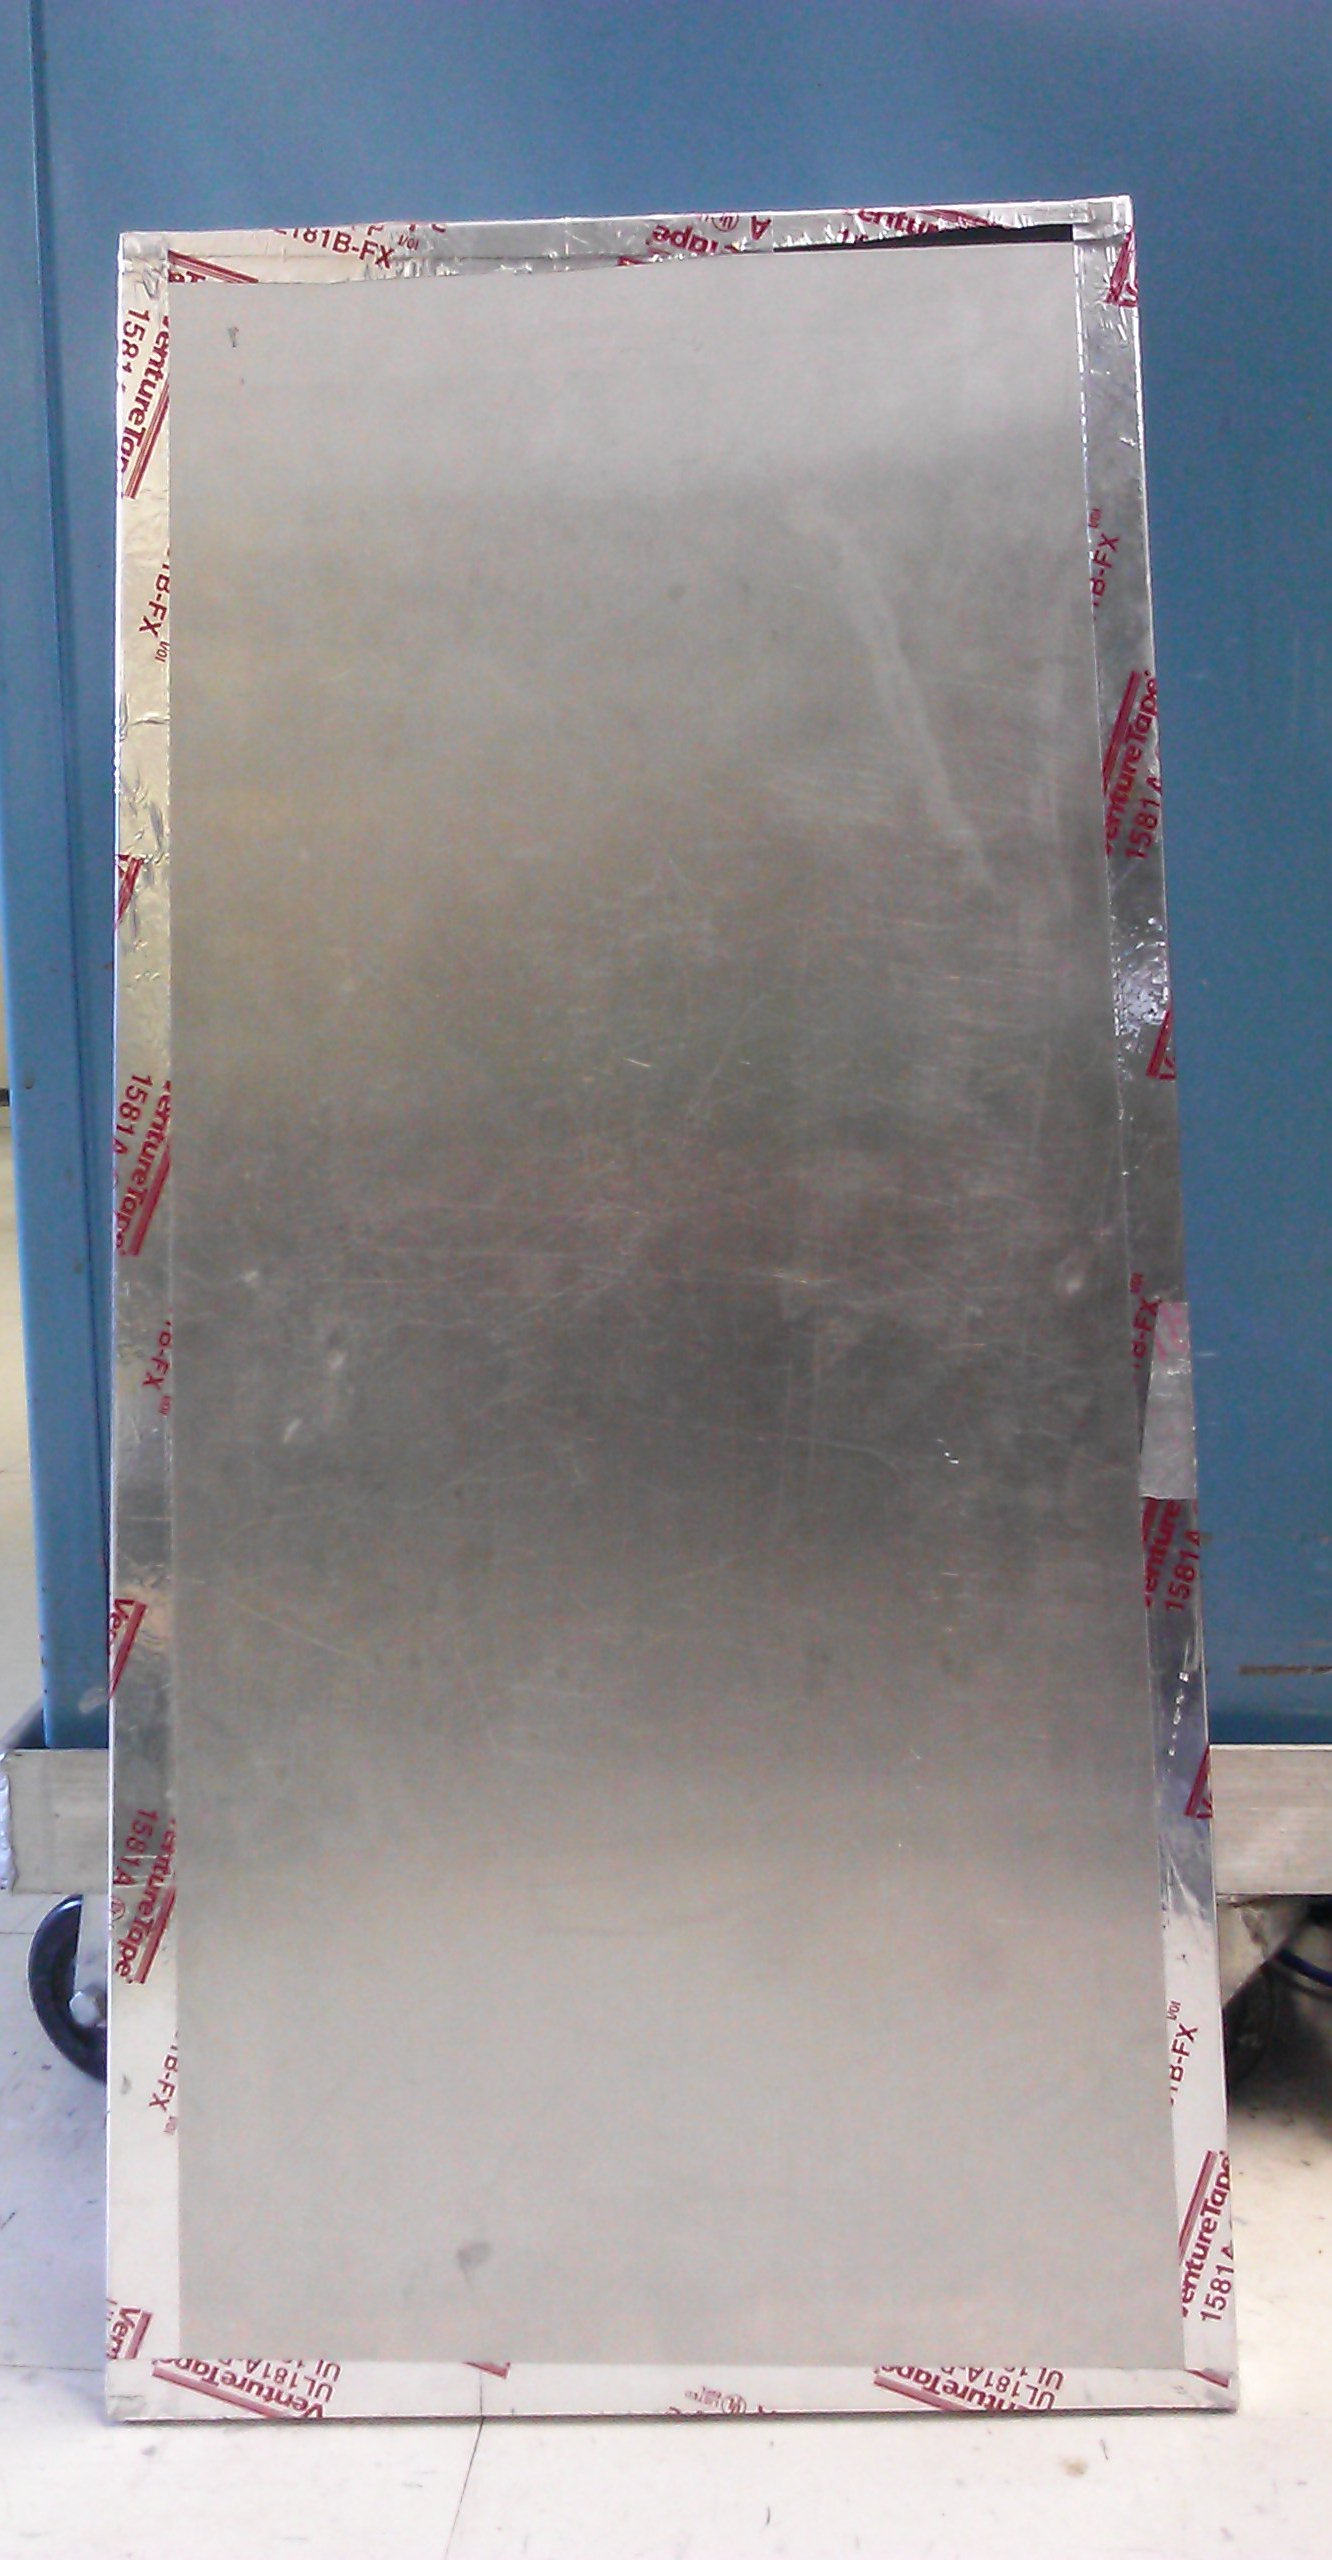
\includegraphics[angle=90,width=0.7\textwidth]{figures/Cosmic_Paddle.jpg}
\caption{
Photograph of one of the scintillation counters used in the cosmic towers. 
} 
\label{pic:cosmicpaddle}
\end{figure}

The paddles were selected from a pool of over 300 scintillating counters collected during the decommissioning of the CDF detector at Fermilab. 
For each counter, both the efficiency $\varepsilon_P$ and the noise $\eta_P$ as a function of the voltage were determined. The measurement was performed sandwiching the given paddle among 4 sample counters, placed two above and two below the paddle under test. The efficiency 
$\varepsilon_P$ was defined as the ratio between the 5-fold coincidence and the 4-fold coincidence of the sample counters. The accidental rate $\eta_P$ was instead defined as the number of 5-fold coincidence observed during ten minutes of data acquisition, when the signal of the paddle under test was delayed by $5 \mu s$. Each paddle with $\varepsilon_P \geq 95\%$ and $\eta_P = 0$ at working voltage was identified as a candidate for the Cosmic Ray system. The ones with the highest efficiency and lowest single count rate were then selected to realize the system itself. 
The plot of $\varepsilon_P$ as a function of the PMT voltage for one example paddle is shown in Fig. \ref{pic:CR_Effplot}.

\begin{figure}[h!]
 \centering
% \includegraphics[width=0.7\textwidth]{figures/TSU29_Efficiency.png}
\caption{
Plot of the counter efficiency $\varepsilon_P$ as a function of the PMT voltage for one of the paddles composing the Cosmic Ray system. 
} 
\label{pic:CR_Effplot}
\end{figure}


%$\varepsilon_P$ at a given voltage is defined as:

%$$
%\varepsilon_P = \frac{R_{1-2} \land R_{3-4} \land R_P}{R_{1-2} \land R_{3-4}}
%$$

%where $R_P$ is the rate of the paddle $P$ to be tested, $R_{1-2}$ is the coincidence rate of two sample paddles positioned above $P$, while $R_{3-4}$ is the coincidence rate of two sample paddles positioned below $P$.
%$\eta_P$ at a given voltage is instead defined as:

%$$
%\eta_P = \frac{R_{1-2} \land R_{3-4} \land R_{P^*}}{R_{1-2} \land R_{3-4}}
%$$

%where $R_{P^*}$ is the Rate of the paddle $P$ 


The trigger rate $R$ of the whole system is $R=0.032Hz$, corresponding to $\sim 1.9~\mu/minute$.
\end{comment}


\chapter{Kaons Interactions in Argon: Cross Section}\label{ch:Interactions}
\section{Literature Review}

%the prediction of the total hadronic interaction cross section ($\pi^{\pm}$, Ar) for thin-target simulations from two Monte Carlo generators (Geant 4.10.1 with Bertini Cascade model~\cite{geant4, g4bert} and Genie v2.8.2 with intranuke-hA model). The thick target simulation used a simple stand-alone Geant4 simulation  (i.e., no other detector features were taken into account except the geometry of the thin slices in the LAr volume). Fig.~\ref{fig:xsplot} shows the resulting total ${\pi^-}$ cross section extracted by the sliced TPC technique; it agrees well with the Geant 4 thin-target cross section. The Genie thin-target cross section for $^{40}$Ar shown in this figure is significantly different than that of Geant at low kinetic energies due to the fact that Geant4 models are tuned on $^{12}$C while Genie ones are tuned on a much heavier $^{56}$Fe target. The extrapolated cross section predicted for $^{40}$Ar can be then very different, especially in the resonance region where the model is strongly target-dependent from one generator to another.
 
%The comparison of the Geant4 thin- and thick-target cross section results demonstrates the power of the "sliced TPC" method for the measurement of the ($\pi^{\pm}$, Ar) cross section in LArIAT TPC geometry. 


%Having validated the ``Sliced TPC'' technique and shown that the this technique recovers the simulated cross-section, we now move to performing this measurement utilizing the complete LArIAT simulation within the LArSoft \cite{} based simulation.  Furthermore, we move from utilizing particle level MC-truth information to performing fully automated reconstruction of the charged hadron events within the LArTPC. 


%Since the kaon cross section in argon has never been measured before, the Geant4 Monte Carlo tunes kaon transportation in argon by extrapolation from lighter and heavier nuclei. As shown in the previous section,  kaon data on carbon are available and  can be used as a metric to evaluate the Geant4 prediction performances.  Figure \ref{fig:TrueCarbon} shows the total hadronic cross section for carbon implemented in Geant4 10.01.p3 overlaid with the Bugg and Friedman data. Unfortunately, the current version of Geant4 does not reproduce the data for carbon closely. On one hand, this evidence makes us even more wary when using the Monte Carlo in simulating the kaon-argon interactions. On the other, it further highlights the importance of kaon measurements.

\section{How to Measure Hadron Cross Section in LArIAT}\label{ch:methodology}
We use both the LArIAT  beamline detectors and the LArTPC information in order to measure hadronic cross sections in argon. Albeit with small differences, both the  $\pi^{-}$-Ar and K$^{+}$-Ar total hadronic cross section measurements rely on the same procedure described in details in the following paragraphs: we select the particle of interest using a combination of beamline detectors and TPC information (paragraph \ref{ch:ParticleSelectionMethod}), we perform a handshake between the beamline information and the TPC tracking to assure we are selecting the right TPC track (paragraph \ref{ch:WC2TPCMatchMethod}), and we apply the ``thin slice" method to get to the final result (paragraph \ref{ch:ThinSliceMethod}).
\subsection{Particle Selection}\label{ch:ParticleSelectionMethod}
\subsection{Wire Chamber to TPC Match}\label{ch:WC2TPCMatchMethod}
After an event passes the selection described in the previous paragraph, we need to identify the track inside the TPC corresponding to the particle which triggered the beamline detectors, a procedure we refer to as ``WC to TPC match". In general, the tracking algorithm will reconstruct more than one track in the event, partially due to the fact that hadrons interact in the chamber, as shown in figure , and partially because of pile up events where the beam of charge particle is too intense compared to the drift time, as shown in figure. 
\textcolor{red}{EVENT DISPLAYS}



\subsection{The Thin Slice Method}\label{ch:ThinSliceMethod}
\subsubsection{Cross Sections on Thin Target}
Cross section measurements on a thin target have been the bread and butter of nuclear and particle {Iexperimentalists since the Rutherford experiments \textcolor{red}{NEED CITATION}. At their core, this type of experiments consists in shooting a beam of particles with a known flux on a thin target and recording the outgoing flux. 


In general, the target is not a single particle, but rather a slab of material containing many diffusion centers. The so-called  ``thin target" approximation assumes that the target centers are uniformly distributed in the material and that the target is thin compared to the interaction length so that no center of interaction sits in front of another. In this approximation, the ratio between the number of particles interacting in the target $N_{Interacting}$ and number of incident particles $N_{Incident}$ determines the interaction probability $P_{Interacting}$, which is the complementary to one of the survival probability $P_{Survival}$. 
Equation \ref{eq:thinTargetXS} 
\begin{equation}
P_{Survival} = 1- P_{Interacting} = 1 - \frac{N_{Interacting}}{N_{Incident}} = e^{-\sigma_{TOT} n \delta X}
\label{eq:thinTargetXS}
\end{equation}
describes the probability for a particle to survive the thin target. This formula relates the total cross section $\sigma_{TOT}$, the density of the target centers  $n$  and  the thickness of the target  along the incident hadron direction $\delta X$, to the interaction probability\footnote{The scattering center density in the target, {\emph{n}},  relates to the argon density $\rho$, the Avogadro number  $ N_{A} $ and the argon molar mass $m_A$ as $n=\frac{\rho N_{A} }{m_A}$.}. If the target is thin compared to the interaction length of the process considered, we can Taylor expand the exponential function in equation \ref{eq:thinTargetXS} and find a simple proportionality relationship between the number of incident and interacting particles, and the cross section, as shown in equation \ref{eq:thinTargetXSTaylor}:
\begin{equation}
1 - \frac{N_{Interacting}}{N_{Incident}} =  1 -\sigma_{TOT} n \delta X + O(\delta X^2).
\label{eq:thinTargetXSTaylor}
\end{equation}

Solving for the cross section, we find:
\begin{equation}
 \sigma_{TOT}  = \frac{1}{n \delta X}\frac{N_{Interacting}}{N_{Incident}}.
\label{eq:thinTargetXSSolved}
\end{equation}

\subsubsection{Not-so-Thin Target: Slicing the Argon}
The LArIAT TPC, with its 90 cm of length, is not a thin target. \textcolor{red}{Find expected interaction length for hadrons and kaons}. However, the fine-grained tracking of the LArIAT LArTPC allows us to treat the argon volume as a sequence of many adjacent thin targets. 

As described in section \ref{sec:experimentDescription}, LArIAT wire planes count 240 wires each. The wires are oriented at +/- $60^{\circ}$ from the vertical direction at 4 mm spacing, while the beam direction is oriented 3 degrees off the $z$ axis in the $XZ$ plane. \textcolor{red}{review this math} The wires collect signals proportional to the energy loss of the hadron along its path in a  $\delta${\emph{X}} = 4 mm/sin($60^{\circ}$) $\approx$ 4.7~mm slab of liquid argon. Thus, one can think to slice the TPC into many thin targets of $\delta${\emph{X}} = 4.7~mm thickness along the direction of the incident particle. 

Considering each slice {\emph{j}}  a ``thin target",  we can apply the cross section calculation from Eq.~\ref{eq:thinTargetXSSolved} iteratively, evaluating the kinetic energy of the hadron as it enters each slice, $E_{j}^{kin}$.  For each WC-to-TPC matched particle, the energy of the hadron entering the TPC is known thanks to the momentum and mass determination by the tertiary beamline, 

\begin{equation}
 E^{kin}_{Front Face}  = \sqrt{p^2_{Beam} - m^2_{Beam}} - E_{loss},
\label{eq:enFF}
\end{equation}
where $E_{loss}$ is a correction for the energy loss in the dead material between the beamline and the TPC front face (more on \ref{sec:Eloss}). The  energy of the hadron at the each slab is determined by subtracting the energy released by the particle in the previous slabs. For example, at the $j^{th}$ point of a track, the kinetic energy will be

\begin{equation}
 E_{j}^{kin} =  E^{kin}_{Front Face} - \sum_{i < j} \Delta E_i,
\label{eq:KEj}
\end{equation}
where $\Delta E_i$ is the energy deposited at each argon slice before the $j^{th}$ point as measured by the calorimetry associated with the tracking.


If the particle enters a slice, it contributes to $N_{Incident}( E^{kin})$ in the energy bin corresponding to its kinetic energy in that slice. If it interacts in the slice, it then also contributes to $N_{Interacting}(E^{kin})$ in the appropriate energy bin. The cross section as a function of kinetic energy, $\sigma_{TOT}( E^{kin})$ will then be proportional to the ratio $\frac{N_{Interacting}( E^{kin})}{N_{Incident}( E^{kin})}$ .


The statistical uncertainty for each energy bin is calculated by error propagation from the statistical  uncertainty on $N_{Incident}$ and $N_{Interacting}$. 
Since the number of incident hadrons in each energy bin is given by a simple counting, we assume that $N_{Incident}$ is distributed as a poissonian with mean and $\sigma^2$ equal to $N_{Incident}$ in each bin.  
On the other hand, $N_{Interacting}$ follows a binomial distribution: a particle in a given energy bin might or might not interact.  The square of the variance for the binomial is given by  
\begin{equation}
\sigma^2 = \mathcal{N}P_{Interacting}(1-P_{Interacting});
\label{eq:binVar}
\end{equation}

since the interaction probability $P_{Interacting}$ is $\frac{ N_{Interacting}}{N_{Incident}}$ and the number of tries $\mathcal{N}$ is $N_{Incident}$, equation \ref{eq:binVar} translates into
\begin{equation}
\sigma^2 = N_{Incident}\frac{ N_{Interacting}}{N_{Incident}} (1-\frac{ N_{Interacting}}{N_{Incident}}) = N_{Interacting}(1-\frac{ N_{Interacting}}{N_{Incident}}).
\end{equation}

$N_{Incident}$ and $N_{Interacting}$ are not independent.
The uncertainty on the cross section is thus calculated as 
\begin{equation}
\delta\sigma_{tot}(E) = \sigma_{tot}(E) \Big(\frac{\delta N_{Interacting}}{N_{Interacting}}+\frac{\delta N_{Incident}}{N_{Incident}}\Big) 
\end{equation}
where:
\begin{eqnarray}
\delta N_{Incident} = \sqrt[]{N_{Incident}} \\
\delta N_{Interacting} = \sqrt[]{N_{Interacting}(1-\frac{ N_{Interacting}}{N_{Incident}})}.
\end{eqnarray}


%%%%%%%%%%%%%%%%%%%%%%%%%%%%%%%%%%%%%%%%%%%%%%%%



\subsection{Procedure testing with truth quantities}
The $\pi^{-}$-Ar and K$^{+}$-Ar total hadronic cross section implemented in Geant4 can be used as a tool to validate the measurement methodology.  We describe here a closure test done on Monte Carlo to prove that the methodology of slicing the TPC retrieves the underlying cross section distribution implemented in Geant4 within the statistical error. %under the working assumption of perfect reconstruction.

For pions in the considered energy range, \textcolor{red}{the Geant4 inelastic model adopted to is ``BertiniCascade", while the elastic model ``hElasticLHEP".}
For kaons, the Geant4 inelastic model adopted to is ``BertiniCascade", while the elastic model ``hElasticLHEP".  


For the validation test, we fire about 390000 pions and 140000 kaons inside the LArIAT TPC active volume using the DDMC (see sec \ref{ch:DDMC}). We apply  the thin-sliced method on using true quantities to calculate the hadron kinetic energy at each slab in order to decouple reconstruction effects to eventual issues with the methodology.  For each slab of 4.7 mm length on the path of the hadron, we integrate the true energy deposition as given by the Geant4 transportation model. Then, we recursively subtracted it from the hadron kinetic energy at the TPC front face to evaluate the kinetic energy at each slab until the true interaction point is reached. Doing so, we obtain the true interacting and incident distributions for the considered hadron and we obtain the true MC cross section as a function of the hadron true kinetic energy. 

Figure \ref{fig:TrueMCXS} shows the total hadronic cross section for argon implemented in Geant4 10.01.p3 (solid lines) overlaid with the true MC cross section as obtained with the sliced TPC method (markers) for pions on the left and kaons on the right; the total cross section is shown in green,  the elastic cross section in blue and the inelastic cross section in red.  The nice agreement with the Geant4 distribution and the cross section  obtained with the sliced TPC method gives us confidence in the  validity of the methodology. 
        
%\begin{comment}     
\begin{figure}
%\captionsetup{justification=raggedright}  
\begin{minipage}[b]{.53\textwidth}  
  \centering  
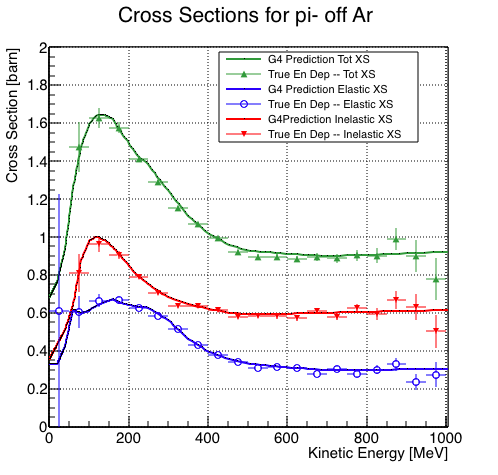
\includegraphics[width=3in]{Chapter-4/Images/PionTrueXS.png}
\end{minipage}%  
\begin{minipage}[b]{0.53\textwidth}  
  \centering  
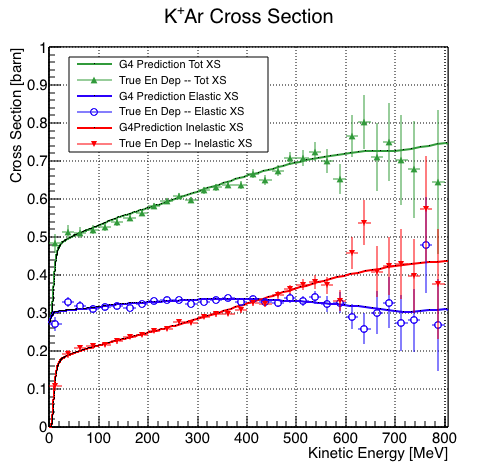
\includegraphics[width=3in]{Chapter-4/Images/KaonTrueXS.png}
\end{minipage}
\label{fig:TrueMCXS}
\caption{Hadronic cross sections for $\pi^-$-Ar (left) and K$^+$-Ar (right) implemented in Geant4 10.01.p3 (solid lines) overlaid the true MC cross section as obtained with the sliced TPC method (markers). The total cross section is shown in green,  the elastic cross section in blue and the inelastic cross section in red.}
%\par
%\begin{minipage}[t]{.53\textwidth}
%\caption{total hadronic cross section for carbon implemented in Geant4  10.01.p3  with overlaid with the Bugg %and Frideman data.}
%\label{fig:TrueCarbon}
%\end{minipage}%
%\begin{minipage}[t]{.5\textwidth}  
%\caption{Hadronic cross sections for argon implemented in Geant4 10.01.p3 (solid lines) overlaid the true MC cross section as obtained with the sliced TPC method (markers). The total cross section is shown in green,  the elastic cross section in blue and the inelastic cross section in red.}
%\label{fig:TrueArgon}
%\end{minipage}  
\end{figure}
%\end{comment}


\subsection{Uncertainty budget}
Measuring an hadronic cross section  in LArIAT translates into counting how many hadrons impinged on a slab of argon at a given energy and how many of those hadrons interacted at said energy. So, the key questions here are:
\begin{itemize}
\item[]a) how well do we know the kinetic energy at each point of the tracking? %(Incident Kinetic Energy bins)
\item[]b) how well do we know when the tracking stops? %(Interacting Kinetic Energy bin)
\item[]c) are there any systematic shifts?
\end{itemize}

In order to answer this question, will discuss first a simple scenario  were our beam is 100\% made of pions which arrive as primaries in the TPC (no decay in the beam and no inelastic interaction before the TPC front face). We will then add a layer of complexity by discussing how we handle beamline contamination.
\subsubsection{Pure beam of pions}
\subsubsection{Handling beamline contamination}
What is the beamline contamination? We define beamline contamination every TPC track matched to the WC track which is not a primary pion. There are 4 different types of beamline contaminations:
\begin{itemize}
\item[]1) electrons,
\item[]2) muons,
\item[]3) secondaries from pion events,
\item[]4) matched pile up events.
\end{itemize}

So, how do we handle this contamination?

The first step is to estimate what percentage of events used in the cross section calculation is not a primary pion.  
We estimate the percentage of electrons and muons in the beam via the beamline MC\footnote{Since the beamline composition is a function of the magnet settings, we simulate separately events for magnet current of -60A and -100A. 
We calculate the electron to pion and muon to pion ratio on the whole sample as the weighted sum of the corresponding ratio in the two current settings, 
\begin{equation}
\frac{N_e}{N_\pi}_{Data} = w_{60A}\frac{N_e}{N_\pi}_{60A}  + w_{100A}\frac{N_e}{N_\pi}_{100A},
\end{equation}
\begin{equation}
\frac{N_\mu}{N_\pi}_{Data} = w_{60A}\frac{N_\mu}{N_\pi}_{60A}  + w_{100A}\frac{N_\mu}{N_\pi}_{100A},
\end{equation}
where the weights $w_{60A}$ and $w_{100A}$ are the percentage of events in the corresponding magnet configuration passing the mass selection in data. }.
Once the beam composition is know,  we simulate the electrons, muons and pions with the DDMC and we subject the three samples to the same selection chain (WC2TPC match, shower filter, pile up filter, etc...). The percentage of electrons and muons surviving the selection chain is the  electron and muon contamination in the pion cross section sample.
The percentage of secondaries is given in the MC by the number of matched WC2TPC tracks which are not flagged as primary by Geant4.
We estimate the last type of contamination, the ``matched pile up" events, to be a negligible fraction, because of the definition of the WC2TPC match: we deem the probability of a single match with a halo particle in the absence of a beamline particle\footnote{ Events with multiple WC2TPC matches are always rejected.} extremely small.


Once we estimate the contaminants to primary pion ratio, the next step is subtracting their contribution from data for each type of contaminant independently. The contaminant samples are reconstructed and the corresponding interacting and incident histograms are produced. We then perform a bin by bin subtraction in the data interacting and incident histograms separately. A graphical rendering of this procedure is shown in Fig \ref{fig:backgroundSubtraction}
Once the data is background subtracted, we apply the correction laid out in the previous section.

\begin{figure}
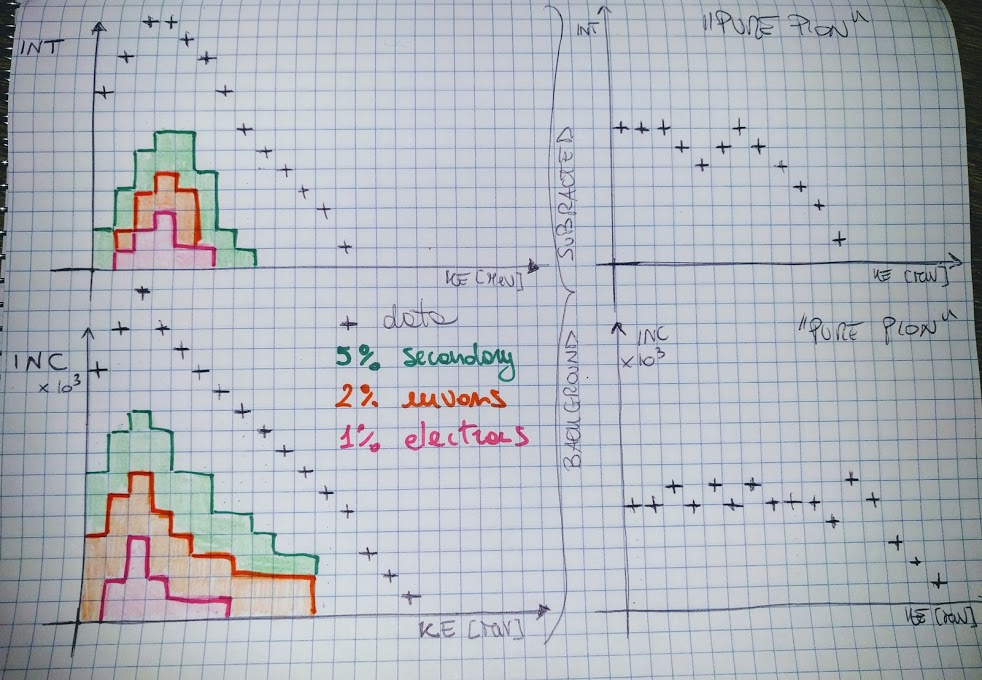
\includegraphics[width=\textwidth,height=\textheight,keepaspectratio]{Chapter-4/Images/FakePlot.jpg}
\label{fig:backgroundSubtraction}
\caption{A graphical rendering of the beamline contamination background subtraction. The contribution of the contaminants is shown in green for the secondaries, in orange for the muons and in pink for electrons. The colored plots are coming from the MC and are staggered. The percentages shown in the legend are the percentages of contaminants over the total number of events  passing the selection chain. We actually expect way less contamination.}
\end{figure}




\chapter{Data Collection}
Your first chapter is probably an introduction. But who knows.
\chapter{LArIAT Monte Carlo}
\section{Beamline}
\subsection{G4Beamline}
\subsection{Data Driven MC}
\label{sec:DDMC}
\section{TPC MC}

\chapter{Energy Calibration}
Your first chapter is probably an introduction. But who knows.
\chapter{Tracking Optimization}
Understanding how kaons and pions are tracked inside the TPC and optimizing the reconstruction algorithms to maximize the correct identification of the interaction point is a fundamental step of the analysis. 


\section{MC sample and WC2TPC match}
The optimization is performed on a MC sample of 191000 kaons and 359000 pions produced with the DDMC technique. DDMC particles are shot from the WC4 location into the TPC following the beam profile.
We mimic the matching between the WC and the TPC track on Monte Carlo by constructing a fake WC track using truth information at wire chamber four. We then apply the same WC to TPC matching algorithm as in data. 

Plots I want in this section:
\begin{enumerate}
\item WC2TPC MC DeltaX, DeltaY and $\alpha$
\item Delta L, reco - true
\item Delta L, reco - true Elastic, Delta L, reco - true Inelastic, other
\item Length Quality cut
\item Efficiency as a function of true KE and Angle
\end{enumerate}





\section{Wire chamber-to-TPC match}
\subsection{Wire chamber-to-TPC match: importance and definition}
\textcolor{red}{something something about why this match is important}

%In data, we attempt to uniquely match one WC-Track to one and only one reconstructed TPC track. This match is done by using in the $X$ and $Y$ coordinate of the extrapolated WC-Track to the upstream most point of the reconstructed TPC Track and by using the angle between the incoming track angle and the reconstructed TPC. We define $\Delta$X as the difference between the $x$ position of the most upstream point of the TPC track and the $x$ position of the WC track as projected to the TPC front face. $\Delta$Y is defined analogously. We define  $\Delta$R as $ \Delta \text{R} =  \sqrt{ \Delta \text{X}^2 +  \Delta \text{Y}^2}  $. The angle between the incident WC Track and the TPC track in the plane that contains them defines $\alpha$.  

%We define a match between WC-track and TPC reconstructed track if  $\Delta \text{R} < r_{T}$, $\alpha < \alpha_{T}$ and the Z position of the first reconstructed point of the TPC track is within 2 cm from the TPC front face. The determination of the best $r_{T}$ and $\alpha_{T}$ is the scope of the following section.

%In MC, we mimic the matching between the WC and the TPC track on Monte Carlo by constructing a fake WC track using truth information at wire chamber four. We then apply the same WC to TPC matching algorithm as in data. 

\subsection{Matching optimization}\label{ch:WC2TPCMatchOptimization}
Scope of this optimization study is assessing the goodness of the wire chamber-to-TPC match on Monte Carlo and porting the optimized selection cuts to data. A word of caution is necessary here. With this study, we want to minimize pathologies associated with the presence of the primary kaon itself, like the incorrect association between the beamline kaon its decay products inside the TPC.  Assessing the contamination from pile-up\footnote{We remind the reader that the DDMC is a single particle Monte Carlo, where the beam pile up is not simulated.}, albeit related, is beyond the scope of this study.

In MC, we are able to define a correct WC2TPC match using the Geant4 truth information. We are thus able to count how many times the WC tracks is associated with the wrong TPC reconstructed track. 

%We define two populations: TPC tracks correctly matched and one of all the other match.
We define a correct match if the all following conditions are met:
\begin{itemize}
\item[-] the length of the true primary Geant4 track in the TPC is greater than 2 cm,  
\item[-] the length of the reconstructed track length is greater than 2 cm,
\item[-] the Z position of the first reconstructed point is within 2 cm from the TPC front face
\item[-] the distance between the reconstructed track and the true entering point is the minimum compared with all the other reconstructed tracks.
\end{itemize}

In order to count the wrong matches, we consider all the reconstructed tracks whose Z position of the first reconstructed point lies within 2 cm from the TPC front face. Events with true length in TPC $<$ 2 cm are included. 
Since kaons are shot 100 cm upstream from the TPC front face, the following two scenarios are possible from a truth standpoint: 
\begin{itemize}
\item[[$Ta$]] the primary kaon decays or interact strongly before getting to the TPC,
\item[[$Tb$]] the primary kaon enters the TPC.
\end{itemize}

Once we choose the selection cuts to determine a reconstructed wire chamber-to-TPC match $r_{T}$ and $\alpha_{T}$, the following four scenarios are possible : 
\begin{itemize}
\item[1)] no reconstructed tracks are matched
\item[2)] the correct track and one (or more) wrong tracks are matched
\item[3)] only the correct track is matched
\item[4)] one (or more) wrong track is matched.
\end{itemize}

If we keep only events with one and only one match, we discard cases 1) and 2) from the cross section measurement. For each set of $r_{T}$ and $\alpha_{T}$ selection value, we define purity and efficiency of the selection as follows:
\begin{equation}
\text{Efficiency} = \frac{\text{Number of events correctly matched}}{\text{ Number of events with primary in TPC}}
\end{equation}

\begin{equation}
\text{Purity} = \frac{\text{Number of events correctly matched}}{\text{Total number of matched events}}.
\end{equation}

Figure \ref{fig:EffPurityK} shows the efficiency (left) and purity (right) for wire chamber-to-TPC match as a function of the radius, $r_{T}$, and angle, $\alpha_{T}$, selection value. It is apparent how both efficiency and purity are fairly flat as a function of the radius selection value at a given angle. This is not surprising, given the fact that the wrong matches can occur  in a single particle gun MC  only for mis-tracking of the primary or for association with decay products, which are generally different in angle, but might be more similar in $x$ and $y$ projection. The radius cut would play a key role in removing pile up events. 

For LArIAT cross section measurements, we generally prefer purity over efficiency, since a sample of particle of a pure species will lead to a better measurement. In the case of kaons however, efficiency needs not to drop too low, given the smallness of the kaon sample. We choose $(\alpha_{T}$, $r_{T}) = (8 \text{ deg}, 4 \text{ cm} )$ and get a MC 85\% efficiency and 98\% purity.


\begin{figure}[hpbt]
\centering
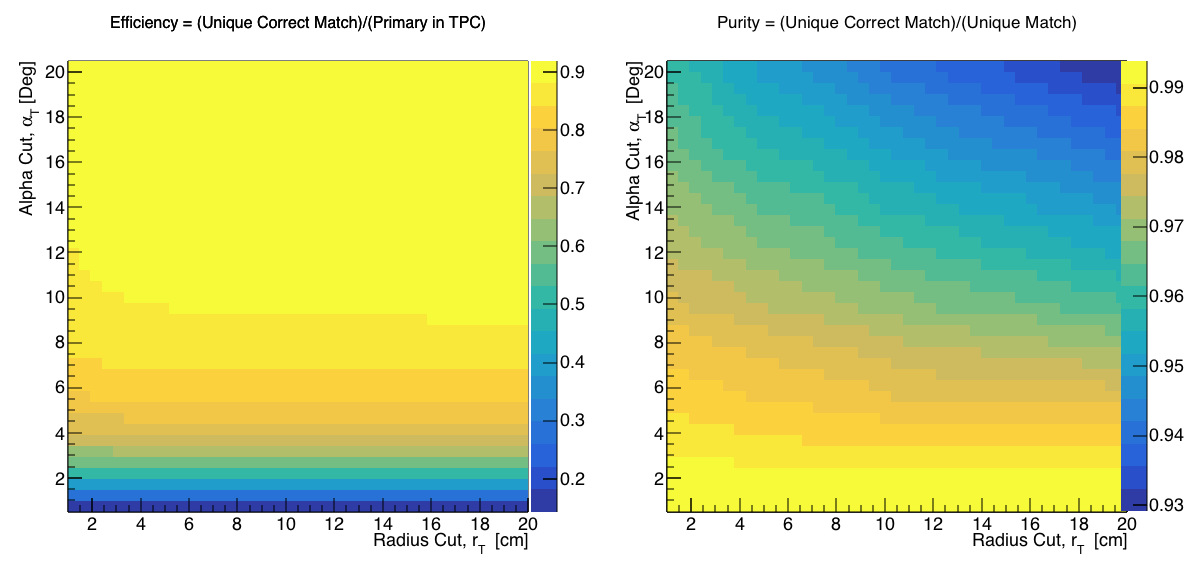
\includegraphics[width=15cm]{Chapter-6/Images/KEffPurity.png}
\caption{Efficiency (left) and purity (right) for wire chamber-to-TPC match as a function of the radius and angle selections.}
\label{fig:EffPurityK}
\end{figure}

\subsection{Porting optimization to data}

\chapter{Kaon Cross Section Measurement}
Your first chapter is probably an introduction. But who knows.


% Add additional \chapter{}s as necessary.

% use \cite{} to cite a reference in your bibliography file.
% use \ref{} to reference a \label{} from an equation, figure, or table.

% for sets of equations use align:
%\begin{align}
%\end{align}

% for figures:
%\begin{figure}[ht]
%\centering
%\includegraphics[width=.45\textwidth]{name_of_figure.eps}
%\caption{A caption! \label{a_figure}}
%\end{figure}

% for tables:
%\begin{table}
%\begin{tabular}{c|c|c}
% 1 & 2 & 3 \\
%\hline
%\end{tabular}
%\caption{Another caption! \label{a_table}}
%\end{table}

% Only call appendix once, here.
\appendix
\chapter{Measurement of LArIAT Electric Field}{ch:AppendixA}
The electric field of a LArTPC in the drift volume is a fundamental quantity for the proper functionality of this technology, as it affects almost every reconstructed quantity such as the position of hits or their collected charge. Given its importance, we calculate the electric field for LArIAT with a single line diagram from our HV circuit and we cross check the obtained value with a measurement relying only on TPC data. 

Before getting into the details of the measurement procedures, it is important to explicit the relationship between some  quantities in play. The electric field and the drift velocity ($v_{drift}$) are related as follows 
\begin{equation} v_{drift} = \mu(E_{field},T) E_{field}, \label{eq:vd}
\end{equation}
where $\mu$ is the electron mobility, which depends on the electric field and on the temperature (T). The empirical formula for this dependency is described in ~\cite{WWW} and shown in Figure \ref{fig:EV} for several argon temperatures.

\begin{figure}[htb]
\centering
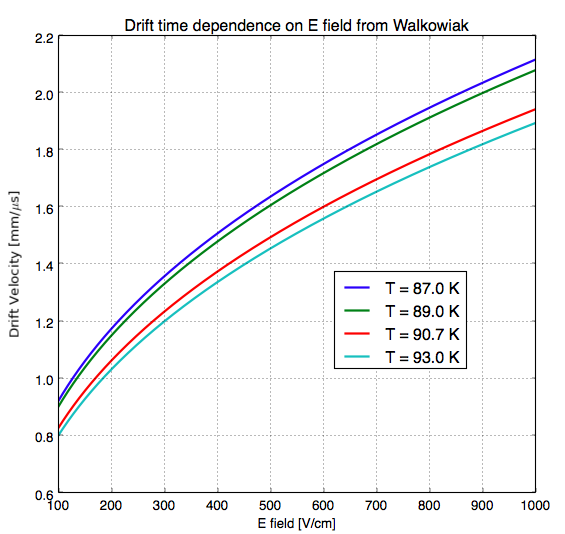
\includegraphics[scale=0.45]{./AppentixA-EField/Images/Walkowiak.png}\\
\caption{Drift velocity dependence on electric field for several temperatures. The slope of the line at any one point represents the electron mobility for that given temperature and electric field.}
\label{fig:EV}
\end{figure}



The relationship between the drift time ($t_{drift}$) and the drift velocity is trivially given by
\begin{equation}
t_{drift} = \Delta x/v_{drift}, \label{eq:drifttime}
\end{equation}
where $\Delta x$ is the distance between the edges of the drift region.
Table \ref{tab:Efields} reports the values of the electric field, drift velocity, and drift times for the smaller drift volumes. 

\begin{table}[]
\centering
\caption{Electric field and drift velocities in LArIAT smaller drift volumes}
\label{tab:Efields}
\begin{tabular}{|l|l|l|}
\hline
& Shield-Induction & Induction-Collection \\ \hline
E$_{filed}$ &                 700.625 V/cm        &                892.5  V/cm             \\ \hline
v$_{drift}$ &                   1.73  mm/$\mu$s   &                  1.90 mm/$\mu$s        \\ \hline
t$_{drift}$ &                   2.31  $\mu$s      &                   2.11 $\mu$s          \\ \hline

\end{tabular}
\end{table}

With these basic parameters established, we can now move on to calculating the electric field in the main drift region (between the cathode and the shield plane).

\subsection*{Single line diagram method}
The electric field strength in the LArIAT main drift volume can be determined knowing the voltage applied to the cathode, the voltage applied at the shield plane, and the distance between them. We assume the distance between the cathode and the shield plane to be 470 mm and any length contraction due to the liquid argon is negligibly small ($\sim$2~mm).

The voltage applied to the cathode can be calculated using Ohm's law and the single line diagram shown in Figure \ref{fig:circuit}.  A set of two of filter pots for emergency power dissipation are positioned between the Glassman power supply and the cathode, one at each end of the feeder cable, each with an internal resistance of 40~M$\Omega$.  The output current of the Glassman power supply is then used to determine the electric field strength.  Figure \ref{fig:currentMeasurement} shows an average current of 0.004172 mA from the Glassman power supply.  

\begin{figure}[h]
\centering
\begin{minipage}{0.45\textwidth}
\centering
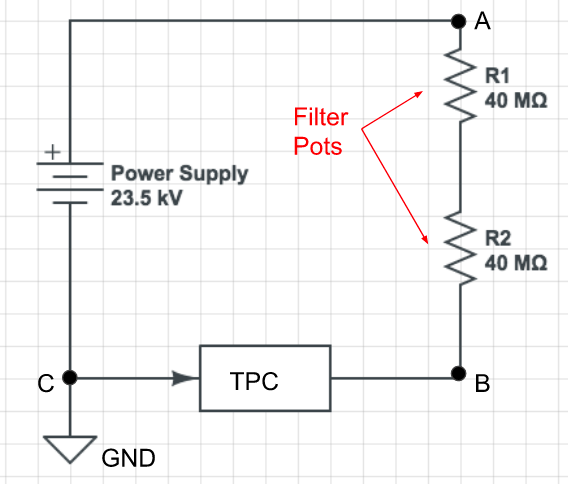
\includegraphics[width=3in]{AppentixA-EField/Images/CircuitLArIAT.png}
\caption{\textcolor{red}{get rid of current line} LArIAT HV simple schematics.}
\label{fig:circuit}
\end{minipage}\hfill
\begin{minipage}{0.45\textwidth}
\centering
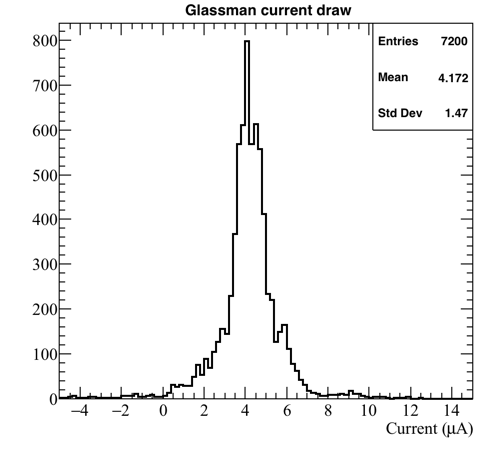
\includegraphics[width=3in]{AppentixA-EField/Images/glassman_current_20160525-30.png}
\caption{\textcolor{red}{the axis is wrong!!} Current reading from the Glassman between May 25th and May 30th, 2016 (typical Run-II conditions).}
\label{fig:currentMeasurement}
\end{minipage}
\end{figure}

Using this current, the voltage at the cathode is calculated as
\begin{equation} \label{eq:VBC}
V_{BC}=V_{PS} - (I \times R_{eq}) = -23.5\text{ kV} + ( 0.00417\text{ mA} \times 80\text{ M}\Omega ) = -23.17\text{ kV}, 
\end{equation}
where $I$ is the current and $R_{eq}$ is the equivalent resistor representing the two filter pots. The electric field, drift voltage, and drift time are then calculated to be
\begin{equation}E_{\text{field}} = \frac{V_{BC} - V_{\text{shield}}}{\Delta x} = 486.54\text{ V/cm}
\end{equation}
%\begin{equation}v_{drift} = \mu E_{field} = 1.5097 \textit{ mm/$\mu$s}
%\end{equation}
%\begin{equation}t_{drift} = \frac{\Delta x}{v_{drift}} = 311.316 \textit{ $\mu$s.}
%\end{equation}



\subsection*{E field using cathode-anode piercing tracks}
%%%%%%%%%%%%%%%%%%%%%%%%%%%%%%%%%%%%%%%%%%%%%%%%%%%%%%%%%%%%%%%%%%%%%%%%%%
\begin{figure}[b]
\centering
\begin{minipage}{0.45\textwidth}
\centering
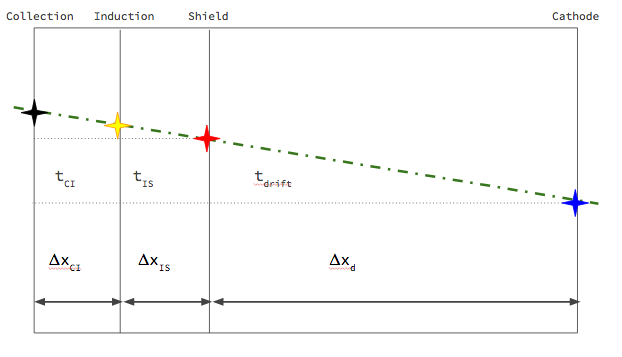
\includegraphics[width=3in]{AppentixA-EField/Images/TPCCrossSectionView.png}
\caption{Pictorial representation of the YX view of the TPC. The distance within the anode planes and between the shield plane and the cathode is purposely out of proportion to illustrate the time difference between hits on collection and induciton. A ACP track is shown as an example.}
\label{fig:Scheme}
\end{minipage}\hfill
\begin{minipage}{0.45\textwidth}
\centering
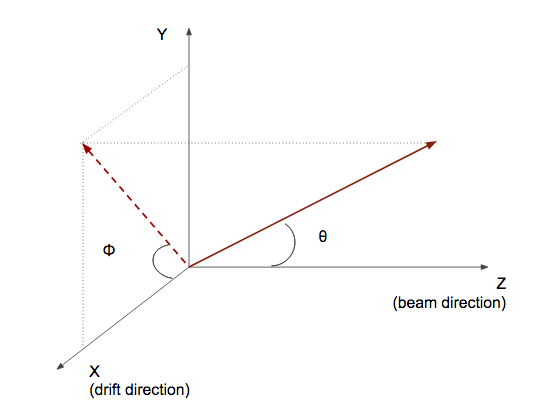
\includegraphics[width=3in]{AppentixA-EField/Images/AngleDef.png}
\caption{Angle definition in the context of LArIAT coordinates system.}
\label{fig:AngleDef}
\end{minipage}
\end{figure}
We devise an independent method to measure the drift time (and consequently drift velocity and electric field) using TPC cathode to anode piercing tracks. We use this method as a cross check to the single line method.
The basic idea is simple:
\begin{itemize}
\item[0.] Select cosmic ray events with only 1 reconstructed track 
\item[1.] Reduce the events to the one contaoning tracks that cross both anode and cathode
\item[2.] Identify the first and last hit of the track
\item[3.] Measure the time difference between these two hits ($\Delta t$).
\end{itemize}
This method works under the assumptions that the time it takes for a cosmic particle to cross the chamber ($\sim$ns) is small compared to the charge drift time ($\sim$ hundreds of $\mu$s).

We choose cosmic events to allow for a high number of anode to cathode piercing tracks (ACP tracks), rejecting  beam  events where the particles travel almost perpendicularly to drift direction. We select events with only one reconstructed track to  maximize the chance of selecting a single crossing muon (no-michel electron). We utilize ACP tracks because their hits span the full drift length of the TPC, see figure \ref{fig:Scheme}, allowing us to define where the first and last hit of the tracks are located in space regardless of our assumption of the electric field. %The definition of the last hit is easy: it is the hit closest to the cathode. The definition of the first hit is a bit more complicated. A track that crosses the anode planes will deposit charge in the small drift volumes (S-I and I-C). The drift time in S-I and I-C region was already calculated in Table \ref{tab:Efields}. This is to say that the position of the first hit matters when calculating the drift time at the microsecond precision. Single hits on the collection plan will not form a 3D object. This means that we can safely exclude that the reconstruction of ACP tracks starts at the cathode plane (black point in figure \ref{fig:Scheme}). %Understanding if the first hit of a track in on the induction or on the shield plan is more complicated. For now, we'll take an uncertainty hit of 2.3 $\mu$s.


One of the main features of this method is that it doesn't rely on the measurement of the trigger time. Since $\Delta t$ is the time difference between the first and last hit of a track and we assume the charge started drifting at the same time for both hits, the measurement of the absolute beginning of drift time $t_0$ is unnecessary. We boost the presence of ACP tracks in the cosmic sample by imposing the following requirements on tracks:

\begin{itemize}
\item vertical position (Y) of first and last hits within $\pm$ 18 cm from TPC center (avoid Top-Bottom tracks) 
\item horizontal position (Z) of first and last hits within 2 and 86 cm from TPC front face (avoid through going tracks) 
\item track length greater than 48 cm (more likely to be crossing)
\item angle from the drift direction (phi in figure \ref{fig:AngleDef}) smaller than 50 deg (more reliable tracking)
\item angle from the beam direction (theta in figure \ref{fig:AngleDef}) grater than 50 deg (more reliable tracking)
\end{itemize}


Tracks passing all these selection requirements are used for the $\Delta t$ calculation.

For each track passing our selection, we loop through the associated hits in order to retrieve the timing information. The analysis is performed separately on hits on the collection plane and induction plane, but lead to consistent results. As an example of the time difference, figures \ref{fig:Run2PosColFit} and \ref{fig:Run2PosIndFit} represent the difference in time between the last and first hit of the selected tracks for Run-II Positive Polarity sample on the collection and induction plane respectively.  We fit with a Gaussian to the peak of the $\Delta t$ distributions to extract the mean drift time and the uncertainty associated with it. The long tail at low $\Delta t$ represent contamination of non-ACP tracks in the track selection.  We apply the same procedure to Run-I and Run-II, positive and negative polarity alike.

   
\begin{figure}[h!]
\begin{minipage}{0.40\textwidth}
\centering
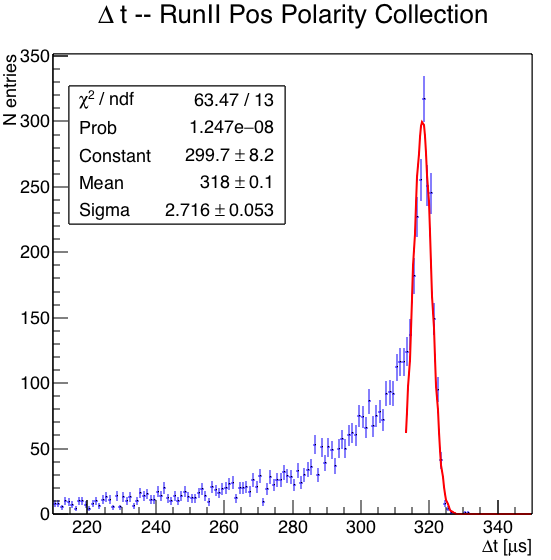
\includegraphics[width=3in]{AppentixA-EField/Images/RunIIPosCol.png}
\caption{Collection plane $\Delta$t fit for Run II positive polarity ACP data  selected tracks.}
\label{fig:Run2PosColFit}
\end{minipage}\hfill
\begin{minipage}{0.40\textwidth}
\centering
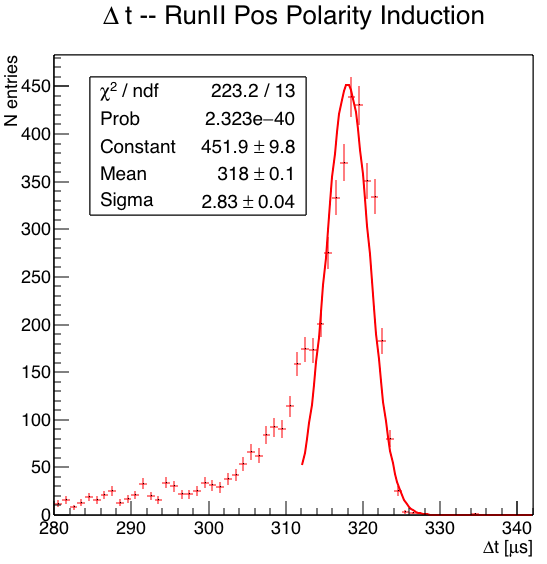
\includegraphics[width=3in]{AppentixA-EField/Images/RunIIPosInd.png}
\caption{Induction plane $\Delta$t fit for Run II positive polarity ACP data  selected tracks.}
\label{fig:Run2PosIndFit}
\end{minipage}
\end{figure}

To convert $\Delta t$ recorded for the hits on the induction plane to the drift time we utilize the formula
\begin{equation}
t_{drift} = \Delta t - t_{S-I}
\end{equation}
where $t_{drift}$ is the time the charge takes to drift in the main volume between the cathode and the shield plane and $t_{S-I}$ is the time it takes for the charge to drift from the shield plane to the induction plane. In Table \ref{tab:Efields} we calculated the drift velocity in the S-I region, thus we can calculate $t_{S-I}$ as 
\begin{equation}
t_{S-I} = \frac{l_{S-I}}{v_{S-I}} = \frac{4 mm}{1.745 mm/ \mu s}
\end{equation}
where $\l_{S-I}$ is the distance between the shield and induction plane and $v_{S-I}$ is the drift velocity in the same region. A completely analogous procedure is followed for the hits on the collection plane, taking into account the time the charge spent in drifting from shield to induction as well as between the induction and collection plane
The value for $\Delta t_{drift}$ , the calculated drift velocity ($v_{drift}$), and corresponding drift electric field for the various run periods is given in Table \ref{tab:deltaTACP} and are consistent with the electric field value calculated with the single line diagram method.

\begin{center}
\begin{table}[htb]
  \begin{center}
    %\resizebox{0.45\textwidth}{!}{%
    \begin{tabular}{|c|c|c|c|}
      \multicolumn{4}{c}{\textbf{Delta t$_{drift}$, drift v and E field with ACP tracks}} \\
      \hline \hline
       Data Period  & $\Delta t_{Drift}$ [$\mu s$] & Drift velocity [mm/$\mu$s] & E field [V/cm] \\
       \hline
       RunI Positive Polarity Induction &  311.1 $\pm$ 2.4   &1.51 $\pm$ 0.01  & 486.6 $\pm$ 21\\
       \hline
       RunI Positive Polarity Collection &  310.9 $\pm$ 2.6 & 1.51 $\pm$ 0.01  &  487.2 $\pm$ 21\\
       \hline
       RunII Positive Polarity Induction &   315.7 $\pm$ 2.8 & 1.49 $\pm$ 0.01 &  467.9 $\pm$ 21\\
       \hline
       RunII Positive Polarity Collection &  315.7 $\pm$ 2.7 & 1.49 $\pm$ 0.01 &  467.9 $\pm$ 21\\
       \hline
       RunII Negative Polarity Induction &   315.9 $\pm$ 2.6 & 1.49 $\pm$ 0.01  & 467.1 $\pm$ 21 \\
       \hline
       RunII Negative Polarity Collection &  315.1 $\pm$ 2.8 & 1.49 $\pm$ 0.01  & 470.3 $\pm$ 21  \\
       \hline
       \hline
       Average Values & 314.1 & 1.50 $\pm$ 0.01 & 474.3 $\pm$ 21 \\
       \hline
       \end{tabular}
    \caption{$\Delta t$ for the different data samples used for the Anode-Cathode Piercing tracks study. }
    \label{tab:deltaTACP}
    \end{center}
\end{table}
\end{center}

%%%%%%%%%%%%%%%%%%%%%%%%%%%%%%%%%%%%%%%%%%%%%%%%%%%%%%%%%%%%




\chapter{Construction of A Cosmic Ray Tagger for MicroBooNE}

\chapter{Pion Analysis}

\subsection{Data Sample}

We decided to use only the data from the  -60 A, -100 A RunII configurations, because the beam composition for these 2 beamline configurations is available in G4Beamline. Run II data is better than Run I in terms of calorimetry and understanding of the detector. 

The used SamWeb definition is PionAna\_RunII\_60A\_100A\_lovely1\_elenag\_00  = 

Defined as ``defname: Lovely1 and data\_tier digits and lariat\_mid\_f\_mc7anb < 0 and create\_date < '2017-06-02' and run\_number != 9276 and run\_number != 9277 and run\_number != 8836 and run\_number != 9083 and run\_number != 9122 and run\_number != 8977 and run\_number != 8981 and run\_number != 8982 and run\_number != 8983 and run\_number != 8984 and run\_number != 8985 and run\_number != 8991 and run\_number != 8994 and run\_number != 8996 and run\_number >= 8767 and
run\_number <= 9635"

\begin{table}[]
\centering
\caption{My caption}
\label{my-label}
\begin{tabular}{|c|c|c|c|}
\hline
Stage                                          & -100A +64 GeV & -60A +64 GeV & Number of Evt \\
\hline
SamWebDefinition                     & 32.7\%        & 67.3\% & 3569206      \\
WCQuality                                  & 37.8\%        & 63.2\% &  553486      \\
P$_{WC4} > $ 420 MeV/c               & 50.8\%        & 49.2\% &  423294      \\
TOF Cut                                     & 32.7\%        & 67.3\% &       \\
\hline
                                               &               &             &\\
\hline
\end{tabular}
\end{table}

\subsection{Capture and Decay}
Our goal is to measure the total hadronic cross section for negative pions in argon. Since pion capture can be classified as an electromagnetic process and pion decay is a week process,  capture and decay represent unwanted interactions in our sample. We present here a study of capture and decay in Monte Carlo and the solution we adopted to mitigate their present in our sample. 

For this MC study, we use a sample of 359000 MC pions generated according to the beam profile with the DDMC described in \ref{sec:DDMC}. Unlike decay -- which may occur both in flight and at rest -- capture occurs predominantly
at rest. Thus, we can highly mitigate capture and decay at rest by removing pions whose energy is low enough to stop in the TPC. This translates into a momentum selection, where we keep only events whose WC momentum is above a certain threshold. 
Figure \ref{fig:CaptureMom} shows the true momentum distribution for the primary\footnote{We use here the Geant4 denomination "primary" to indicate that the pion considered does not undergo interactions modifying its energy before getting to the TPC. In fact, not every pion shot from wire chamber four will arrive to the TPC as primary,  some will decay or interact before the TPC, as explained in \textcolor{red}{reference to WC 2 TPC chapter}} pions that arrive to the TPC (pink), that capture (green) or decay (blue) inside the TPC, on a linear and log scale vertical axis. 

\begin{figure}[hpbt]
\centering
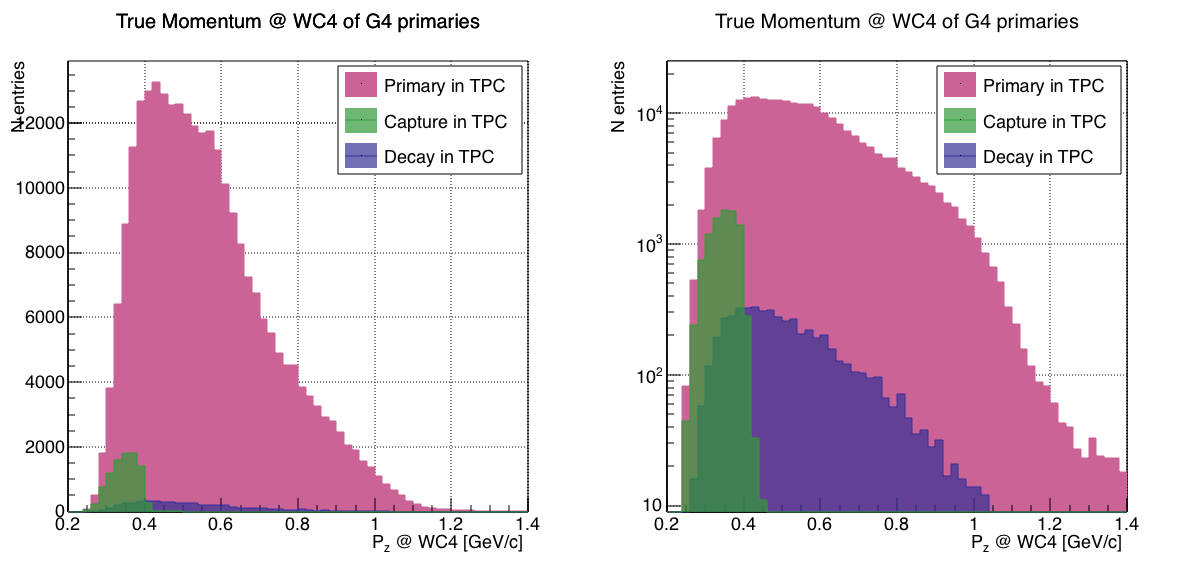
\includegraphics[width=15cm]{Chapters/C-PionImages/CDAsMomentumFunct.png}
\caption{True momentum distribution at wire chamber 4 for every simulated pion arriving in the TPC (pink), ending its life in capture (green) or in decay (blue) in the TPC, linear vertical axis on the left, logarithmic on the right. }
\label{fig:CaptureMom}
\end{figure}


In order to choose the selection value for the wire chamber momentum, it is beneficial to estimate the ratio of events which capture or decay that survive the selection in MC as a function of the momentum threshold, and compare it with the survival ratio for all events. This is done in figure \ref{fig:survRatio}. We define the survival ratio simply  as the number of events surviving the true momentum cut divided by the number of events of that given category. The survival ratio calculated separately for the three event categories explained above: total (pink), capture (green) and decay (blue).
Selecting pions with momentum greater than 420 MeV/c reduces the capture events by ~99\% while maintaining about 80\% of the total data sample. 
Figure \ref{fig:evtRatio} shows the ratio of events which end their life in capture (green) or decay (blue) over the total number of events as a as a function of the true momentum at wire chamber four. This ratio is slightly dependent on the inelastic cross section implemented in Geant4, as we are able to register a pion capture (or decay) only if it doesn't interact inelastically in the TPC. For momenta greater than 420 MeV/c, the percentage of capture events drops below 1\% and the percentage of decays is never above 2\%.

\begin{figure}[h!]
\centering
\begin{minipage}[t]{0.45\textwidth}
\centering
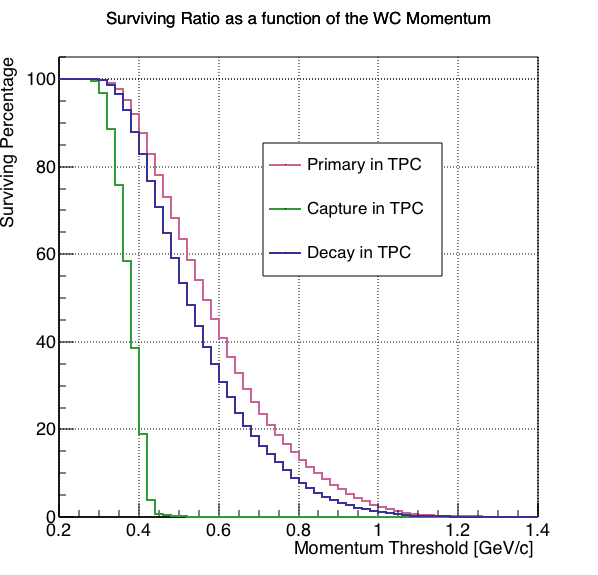
\includegraphics[width=7.5cm]{Chapters/C-PionImages/CDThreshold.png}
\caption{Survival ratio as a function of selection threshold on true momentum at wire chamber four for for every simulated pion arriving in the TPC (pink), capture (green) or in decay (blue).   }
\label{fig:survRatio}
\end{minipage}\hfill
\begin{minipage}[t]{0.45\textwidth}
\centering
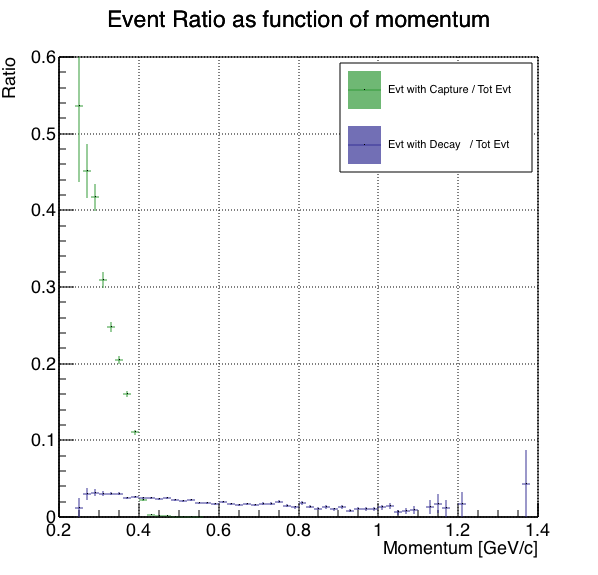
\includegraphics[width=7.5cm]{Chapters/C-PionImages/CDRatio.png}
\caption{Ratio between the capture (green) and decay (blue) events over the total number of events as a as a function of the true momentum at wire chamber four.}
\label{fig:evtRatio}
\end{minipage}
\end{figure}















% Any chapters such as End Notes go after this.
\backmatter

\bibliography{bib.bib}
\bibliographystyle{plain}
% for your own sake, use a bibtex file, so all of the numbering of references will be done
% automatically.

\end{document}
